\documentclass[12pt,letterpaper]{article}

% --- Paquetes Fundamentales ---
\usepackage[spanish,es-tabla,es-noquoting]{babel}
\usepackage[utf8]{inputenc}
\usepackage[T1]{fontenc}
\usepackage{lmodern}
\usepackage{geometry}
\geometry{
    top=2.54cm,
    bottom=2.54cm,
    left=2.54cm,
    right=2.54cm,
    headheight=15pt
}

% --- Paquetes Matemáticos y Científicos ---
\usepackage{amsmath,amssymb,amsfonts,amsthm}
\usepackage{bm}
\usepackage{enumitem}
\usepackage[round,authoryear]{natbib}

% --- Paquetes de Tablas y Formato ---
\usepackage{booktabs}
\usepackage{tabularx}
\usepackage{longtable}
\usepackage{array}
\usepackage{multirow}
\usepackage{colortbl}

% Columnas personalizadas para tabularx con alineación controlada
\newcolumntype{L}{>{\raggedright\arraybackslash}X}
\newcolumntype{C}{>{\centering\arraybackslash}X}
\newcolumntype{R}{>{\raggedleft\arraybackslash}X}

% --- Formato APA 7 para Títulos de Tablas y Figuras ---
\usepackage{caption}
\captionsetup[table]{
    labelfont=bf,
    textfont=it,
    labelsep=newline,
    justification=raggedright,
    singlelinecheck=false
}
\captionsetup[figure]{
    labelfont=bf,
    textfont=it,
    labelsep=newline,
    justification=raggedright,
    singlelinecheck=false
}

% --- Gráficos, Colores y Diagramas ---
\usepackage{graphicx}
\graphicspath{{figuras/}{../static/img/}}
\usepackage{xcolor}
\usepackage{tikz}
\usetikzlibrary{shapes.geometric, arrows, arrows.meta, positioning, calc, trees, shadows, fit, backgrounds, babel}

% Definición de Colores Institucionales y de Acento
\definecolor{primaryblue}{RGB}{24, 76, 120}
\definecolor{secondaryblue}{RGB}{41, 128, 185}
\definecolor{darkgray}{RGB}{50, 50, 50}
\definecolor{lightgray}{RGB}{245, 247, 250}
\definecolor{tableheader}{RGB}{220, 230, 242}
\definecolor{accentgreen}{RGB}{39, 174, 96}
\definecolor{accentorange}{RGB}{211, 84, 0}
\definecolor{accentred}{RGB}{192, 57, 43}

% --- Cajas y Énfasis ---
\usepackage[many]{tcolorbox}
\newtcolorbox{resumenbox}{
    colback=lightgray,
    colframe=primaryblue,
    arc=3mm,
    boxrule=1.2pt,
    left=12pt,
    right=12pt,
    top=8pt,
    bottom=8pt
}

\newtcolorbox{interpretacionbox}{
    colback=white,
    colframe=secondaryblue!70!black,
    arc=2mm,
    boxrule=0.8pt,
    fonttitle=\bfseries\small,
    coltitle=white,
    title=Interpretación Técnica y Práctica,
    left=10pt,
    right=10pt,
    top=8pt,
    bottom=8pt
}

% --- Encabezados y Pies de Página según APA 7 ---
\usepackage{fancyhdr}
\pagestyle{fancy}
\fancyhf{}
\fancyhead[L]{\small\color{darkgray}\textit{Minería Web}}
\fancyhead[R]{\small\thepage}
\fancyfoot{}
\renewcommand{\headrulewidth}{0.4pt}
\renewcommand{\footrulewidth}{0pt}

% --- Macros de Notas de Tablas y Figuras en Estándar APA 7 ---
\newcommand{\tablenote}[1]{%
    \vspace{2mm}%
    \begin{minipage}{\linewidth}%
        \footnotesize\textit{Nota.} #1%
    \end{minipage}%
}
\newcommand{\figurenote}[1]{%
    \vspace{2mm}%
    \begin{minipage}{\linewidth}%
        \footnotesize\textit{Nota.} #1%
    \end{minipage}%
}

% --- Títulos de Secciones ---
\usepackage{titlesec}
\titleformat{\section}
    {\normalfont\Large\bfseries\color{primaryblue}}{\thesection.}{0.8em}{}
\titleformat{\subsection}
    {\normalfont\large\bfseries\color{secondaryblue}}{\thesubsection.}{0.6em}{}
\titleformat{\subsubsection}
    {\normalfont\normalsize\bfseries\itshape\color{darkgray}}{\thesubsubsection.}{0.5em}{}

% --- Hipervínculos ---
\usepackage{hyperref}
\usepackage{xurl}
\hypersetup{
    colorlinks=true,
    linkcolor=primaryblue,
    citecolor=secondaryblue,
    urlcolor=secondaryblue,
    pdftitle={Sistema Integral de Minería Web Multidimensional para el Monitoreo de Precios, Salud y Contrataciones en Bolivia},
    pdfauthor={Univ. Julio Nelson Arias Cruz},
    pdfsubject={Minería de Datos - Web Mining},
    pdfkeywords={Web Mining, Web Content Mining, Web Structure Mining, Web Usage Mining, PageRank, HITS, Scraping Resiliente, Neon PostgreSQL, Next.js, Telegram Bot}
}
\emergencystretch=3em
\tolerance=2000

% --- Entornos de Código ---
\usepackage{listings}
\lstset{
    basicstyle=\ttfamily\footnotesize,
    breaklines=true,
    frame=single,
    backgroundcolor=\color{lightgray},
    keywordstyle=\color{primaryblue}\bfseries,
    commentstyle=\color{gray}\itshape,
    stringstyle=\color{accentgreen},
    numbers=left,
    numberstyle=\tiny\color{darkgray},
    stepnumber=1,
    tabsize=2,
    showstringspaces=false
}
\lstdefinelanguage{json}{
    basicstyle=\ttfamily\footnotesize,
    string=[s]{"}{"},
    stringstyle=\color{accentgreen},
    comment=[l]{:},
    commentstyle=\color{primaryblue}\bfseries,
    keywords={true, false, null},
    keywordstyle=\color{accentorange}\bfseries
}

\setlength{\parindent}{1.27cm}
\setlength{\parskip}{0pt}

\begin{document}

% ----------------------------------------------------
% PORTADA INSTITUCIONAL
% ----------------------------------------------------
\begin{titlepage}
    \centering
    \vspace*{0.2cm}
    
    {\fontsize{15}{18}\selectfont \textbf{UNIVERSIDAD MAYOR DE SAN ANDRÉS}}\\[0.25cm]
    {\fontsize{13}{16}\selectfont \textbf{FACULTAD DE CIENCIAS PURAS Y NATURALES}}\\[0.2cm]
    {\fontsize{13}{16}\selectfont \textbf{CARRERA DE INFORMÁTICA}}\par
    
    \vspace{0.4cm}
    
    % Emblema Institucional Oficial UMSA
    
\includegraphics[height=8cm, keepaspectratio]{figuras/logo_umsa.png}
    
    \vspace{0.4cm}
    
    {\fontsize{11}{14}\selectfont \textbf{INFORME FINAL}}\\[0.3cm]
    
    % Título oficial del proyecto en formato APA 7
    {\fontsize{13}{17}\selectfont \textbf{SISTEMA INTEGRAL DE MINERÍA WEB MULTIDIMENSIONAL (CONTENIDO, ESTRUCTURA Y USO) PARA EL MONITOREO DE PRECIOS RETAIL, SALUD CIUDADANA Y CONTRATACIONES ESTATALES EN BOLIVIA}}\par
    
    \vspace{0.6cm}
    
    {\fontsize{11}{14}\selectfont \textbf{AUTOR:}}\\[0.15cm]
    {\fontsize{12}{15}\selectfont \textbf{Univ. Julio Nelson Arias Cruz}}\par
    
    \vspace{0.5cm}
    
    {\fontsize{10}{13}\selectfont
    \textbf{Bot Telegram:} \url{https://t.me/ChatDM7200bot}\\[0.12cm]
    \textbf{Plataforma Web} \url{https://ws-dm.vercel.app/} \\
    \textbf{Repositorio Github} \url{https://github.com/JulioArias7200/ws-dm} 
    }
    
    \vfill
    
    {\fontsize{11}{14}\selectfont \textbf{ASIGNATURA:} Minería de Datos}\\[0.15cm]
    {\fontsize{11}{14}\selectfont \textbf{DOCENTE:} M.Sc. Menfy Morales Rios}\\[0.2cm]
    {\fontsize{11}{14}\selectfont La Paz -- Bolivia, Noviembre 2026}
    
    \vspace*{0.2cm}
\end{titlepage}


% ----------------------------------------------------
% TABLA DE CONTENIDO E ÍNDICES SEGÚN APA 7
% ----------------------------------------------------
\newpage
\pagenumbering{roman}
\setcounter{page}{2}
\phantomsection
\addcontentsline{toc}{section}{ÍNDICE GENERAL}
\tableofcontents

\newpage
\phantomsection
\addcontentsline{toc}{section}{ÍNDICE DE FIGURAS}
\listoffigures

\newpage
\phantomsection
\addcontentsline{toc}{section}{ÍNDICE DE TABLAS}
\listoftables

\newpage
\pagenumbering{arabic}
\setcounter{page}{1}

% ----------------------------------------------------
% SECCIONES ESTRUCTURALES DEL INFORME
% ----------------------------------------------------
\section{INTRODUCCIÓN}

El crecimiento acelerado de las plataformas de comercio electrónico y los portales de gestión pública en Bolivia ha configurado un entorno digital caracterizado por una alta densidad de datos. No obstante, a diferencia de otros ecosistemas internacionales consolidados, el ámbito digital boliviano presenta una marcada asimetría informativa y una notable opacidad en la publicación de datos abiertos estructurados. Las principales cadenas de retail minorista y cadenas farmacéuticas del país carecen de interfaces de programación de aplicaciones (API) públicas y accesibles para la ciudadanía o la comunidad académica. Esta limitación restringe la capacidad de monitorear oportunamente la fluctuación de precios de la canasta familiar y evaluar la dispersión de costos de medicamentos esenciales en los centros urbanos del eje central: La Paz, Cochabamba y Santa Cruz.

De manera simultánea, las plataformas gubernamentales como el Sistema de Contrataciones Estatales (SICOES) y el Observatorio Agroambiental y Productivo (OAP) concentran volúmenes sustanciales de convocatorias públicas y series de abastecimiento agropecuario. Sin embargo, su consumo automatizado se ve obstaculizado por esquemas de búsqueda tradicionales basados exclusivamente en concordancia exacta de cadenas de texto y arquitecturas web protegidas por cortafuegos de aplicaciones web (WAF, por sus siglas en inglés).

Para responder a estos desafíos tecnológicos y sociales, el presente proyecto académico desarrolla e implementa un \textbf{Sistema Integral de Minería Web Multidimensional}, articulando de manera armónica las tres ramas clásicas de la disciplina conceptualizadas por \citet{liu2011web} y \citet{han2012data}:

\begin{enumerate}[leftmargin=*, label=\textbf{\arabic*.}]
    \item \textbf{Minería de Contenido Web (\textit{Web Content Mining}):} Construcción y despliegue de agentes de extracción automatizada y resiliente basados en Node.js y Playwright, diseñados para superar barreras dinámicas de representación del lado del cliente (\textit{Client-Side Rendering}), desplazamiento infinito (\textit{infinite scrolling}) y mecanismos de protección perimetral basados en desafíos biométricos y de comportamiento humano (WAF Radware Bot Manager y hCAPTCHA). Este subsistema opera sobre los catálogos en línea de Hipermaxi, Farmacorp, Farmacias Chávez, el portal de licitaciones de SICOES y el observatorio de precios del OAP.
    
    \item \textbf{Minería de Estructura Web (\textit{Web Structure Mining}):} Extracción, modelado y análisis de la topología de red de contrataciones estatales en el departamento de La Paz. El sistema construye grafos bipartitos dirigidos conectando entidades públicas convocantes con rubros comerciales y proveedores adjudicados, aplicando formalmente los algoritmos \textbf{PageRank} \citep{page1998anatomy} y \textbf{HITS} (\textit{Hyperlink-Induced Topic Search}) \citep{kleinberg1999authoritative} para identificar concentraciones de poder licitador y autoridades temáticas en compras públicas.
    
    \item \textbf{Minería de Uso Web (\textit{Web Usage Mining}):} Instrumentación de telemetría de eventos, tiempos de respuesta y patrones de interacción humana mediante el asistente conversacional oficial desplegado en Telegram (\texttt{@ChatDM7200bot}) \citep{srivastava2000web, cooley1999data}. Se capturan trazas operacionales para optimizar la navegación faceted de los usuarios y enriquecer los flujos de consulta en lenguaje natural.
\end{enumerate}

El ecosistema integra una arquitectura de datos en la nube sobre \textbf{Neon Serverless PostgreSQL}, estructurada mediante un modelo estrella relacional que combina un catálogo maestro inmutable de productos (\textit{Master Catalog}), series de tiempo particionadas de forma declarativa por rangos mensuales (\textit{Time-Series Partitioning}) y triggers reactivos PL/pgSQL que calculan en tiempo de inserción las variaciones de precio ($\Delta\text{Bs}$ y $\Delta\%$). Adicionalmente, el pipeline multimedia desacopla los activos visuales efímeros de las plataformas origen mediante un almacenamiento persistente en \textbf{Neon Object Storage S3}, sirviendo los activos a través de una plataforma web interactiva construida en \textbf{Next.js 14} y complementada con búsqueda semántica vectorial densa impulsada por modelos de inteligencia artificial \textbf{NVIDIA NIM} (1024 dimensiones) y cartografía geoespacial con \textbf{OpenStreetMap}.

El presente informe detalla el marco teórico, metodológico y práctico del proyecto, exponiendo el diseño arquitectónico, las evidencias visuales y las métricas de rendimiento auditadas en el entorno operativo.

\section{ANTECEDENTES}

\subsection{Recolección de Precios y Monitoreo de Mercado en Bolivia}
Históricamente, el seguimiento de la dinámica de precios al consumidor en el territorio boliviano ha dependido fundamentalmente de relevamientos presenciales coordinados por entidades gubernamentales. El Instituto Nacional de Estadística (INE) fundamenta la estimación del Índice de Precios al Consumidor (IPC) en operativos de campo periódicos en mercados zonales y ferias francas. Por su parte, el Ministerio de Desarrollo Rural y Tierras administra el Observatorio Agroambiental y Productivo (OAP), cuyo objetivo es documentar el comportamiento de precios en origen y en mercados mayoristas para salvaguardar la soberanía y seguridad alimentaria.

El portal oficial del OAP provee un sistema de consulta de precios orientado a productos agrícolas e insumos de la canasta básica. No obstante, su estructura está concebida primordialmente para el consumo visual humano mediante formularios web tradicionales, careciendo de mecanismos de interoperabilidad, servicios web REST o endpoints JSON abiertos que posibiliten el análisis automatizado y continuo de series de tiempo.

\subsection{El Portal de Contrataciones Estatales (SICOES)}
En el ámbito de las compras del Estado boliviano, el Sistema de Contrataciones Estatales (SICOES) es el órgano rector digital establecido bajo el marco del Decreto Supremo N.º 0181 (Normas Básicas del Sistema de Administración de Bienes y Servicios - NB-SABS). Dicho portal concentra los procesos licitatorios de entidades centralizadas, descentralizadas, gobernaciones departamentales y gobiernos autónomos municipales.

A pesar de su trascendencia cívica y económica, el motor de búsqueda del SICOES presenta severas limitaciones de recuperación de información (\textit{Information Retrieval}). El sistema opera bajo concordancias estrictas de subcadenas alfanuméricas sobre el Código Único de Contratación Estatal (CUCE) o el objeto textual declarado. Esto impide la recuperación semántica de convocatorias cuando los términos empleados en los pliegos difieren sintácticamente de la consulta ciudadana (por ejemplo, buscar ``suministro de reactivos de laboratorio'' no retorna licitaciones redactadas como ``adquisición de insumos de diagnóstico clínico''). Asimismo, la plataforma no provee un modelado de redes que vincule las entidades licitantes con sus proveedores recurrentes o consorcios empresariales.

\subsection{Evolución Tecnológica de las Plataformas Web y el Auge de los WAF}
En la última década, las principales corporaciones de comercio retail y farmacéutico de Bolivia modernizaron sus plataformas digitales, transitando desde sitios basados en HTML estático hacia aplicaciones de una sola página (\textit{Single Page Applications} - SPAs) y arquitecturas híbridas renderizadas en servidor (\textit{Server-Side Rendering} - SSR), construidas sobre frameworks como React, Next.js y ecosistemas de e-commerce como Shopify.

Simultáneamente, con el propósito de mitigar ataques distribuidos de denegación de servicio (DDoS) y prevenir la indexación masiva por terceros, las empresas incorporaron cortafuegos de aplicaciones web de última generación (\textit{Next-Generation WAF}), entre los que destaca \textbf{Radware Bot Manager} \citep{radware2024}. Estos sistemas implementan análisis biométrico pasivo, verificación de huella digital de navegador (\textit{browser fingerprinting}) y retos dinámicos de captcha (\textit{hCAPTCHA}), tornando obsoletos a los scrapers tradicionales basados en peticiones HTTP primitivas (como \texttt{curl}, \texttt{requests} o \texttt{cheerio}). Ante este escenario, la investigación en Minería Web demanda la adopción de navegadores automatizados controlados mediante protocolos CDP (\textit{Chrome DevTools Protocol}) y estrategias de persistencia de perfiles de usuario.

\section{PLANTEAMIENTO DEL PROBLEMA}

\subsection{Descripción del Problema y Asimetría de Mercado}
En el mercado boliviano de bienes de consumo masivo y productos farmacéuticos coexiste una marcada fragmentación de precios. El consumidor promedio se enfrenta a variaciones sustanciales en el costo final de un mismo producto dependiendo de la cadena comercial, la ubicación geográfica de la sucursal o el canal de venta (físico o digital). En el rubro farmacéutico, esta asimetría adquiere especial gravedad: medicamentos esenciales como el \textit{Paracetamol 500 mg}, el \textit{Ibuprofeno 400 mg} o el \textit{Losartán 50 mg} pueden registrar diferenciales de precio superiores al 100\% entre cadenas competidoras o incluso entre presentaciones de marca e insumos genéricos. 

La falta de herramientas centralizadas y públicas que comparen estas variaciones en tiempo real genera ineficiencias en el gasto familiar e incrementa los costos de búsqueda para los ciudadanos, quienes deben visitar manualmente múltiples sucursales o navegar portales web desconectados entre sí.

\subsection{Vulnerabilidad de los Mecanismos de Extracción Tradicionales}
La recolección masiva de datos en la web moderna enfrenta obstáculos técnicos de alta complejidad. La mayoría de los supermercados y farmacias han adoptado esquemas de renderizado dinámico en el cliente y mecanismos de defensa automatizados contra bots. Como se ilustra en la Figura~\ref{fig:radware_challenge}, plataformas como Hipermaxi implementan capas de seguridad perimetral provistas por \textbf{Radware Bot Manager}, las cuales interceptan las conexiones automáticas y despliegan desafíos interactivos de tipo \textit{hCAPTCHA} cuando detectan firmas sintéticas o ausencia de interacción táctil o de puntero humano.

\begin{figure}[htbp]
    \centering
    \caption{Desafío de Verificación Humana de Radware Bot Manager en Plataforma Hipermaxi}
    \label{fig:radware_challenge}
    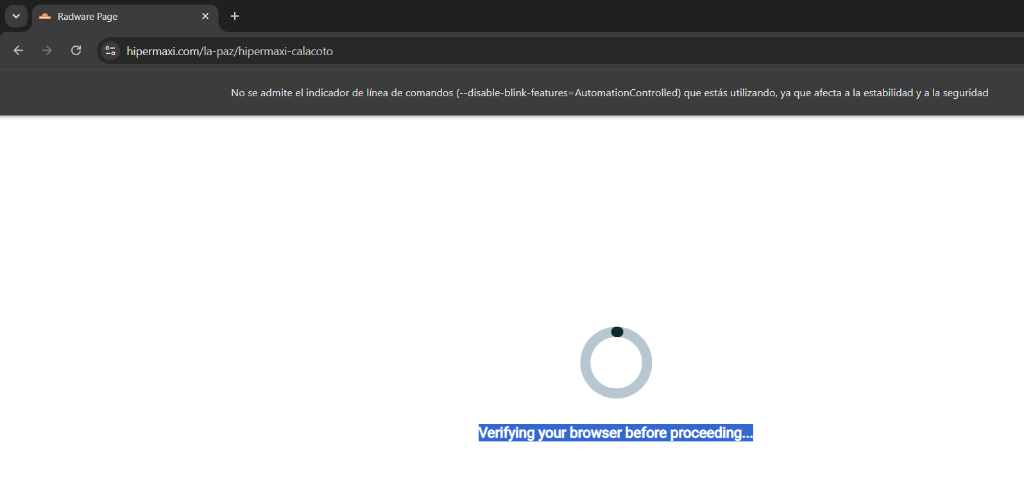
\includegraphics[width=0.85\linewidth]{figuras/radware_bot_manager_challenge.png}
    \figurenote{Pantalla de intercepción de tráfico emitida por Radware Bot Manager en el portal de Hipermaxi Bolivia. Demuestra el bloqueo inmediato de scrapers no instrumentados y justifica la necesidad de utilizar navegadores reales con perfiles persistentes y emulación de interacción humana.}
\end{figure}

Cuando los bots automatizados persisten en peticiones recurrentes sin almacenar estado o fallan al responder los desafíos criptográficos iniciales de JavaScript, Radware escala la protección hacia un segundo nivel más restrictivo: la pantalla de detección de anomalías con reto interactivo \textit{hCaptcha} (Figura~\ref{fig:radware_captcha}).

\begin{figure}[htbp]
    \centering
    \caption{Intercepción Activa de Radware Bot Manager con Desafío hCaptcha ante Anomalías}
    \label{fig:radware_captcha}
    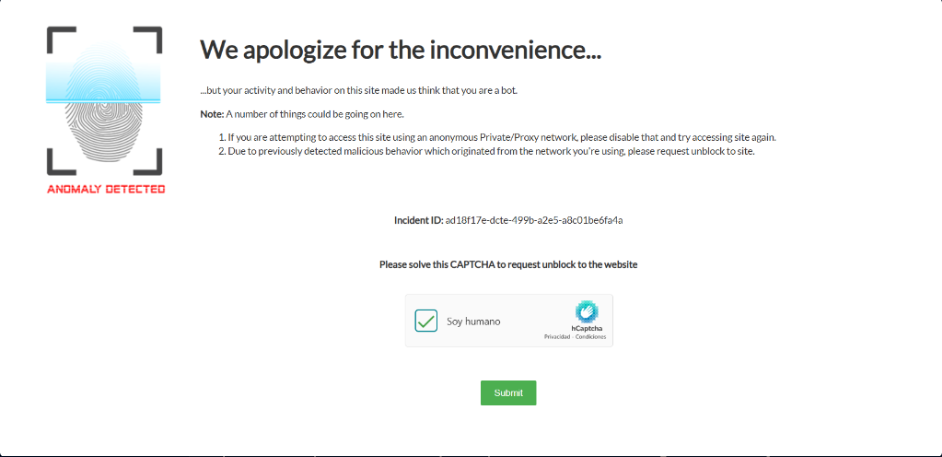
\includegraphics[width=0.85\linewidth]{figuras/imgADVERTENCIA1.png}
    \figurenote{Respuesta perimetral de Radware Bot Manager al detectar anomalías en la firma de navegación o patrones automatizados. Demuestra la escalada hacia retos interactivos de verificación humana (\textit{hCaptcha}) que invalidan los scrapers basados en peticiones HTTP estáticas.}
\end{figure}

A este blindaje perimetral se añade la complejidad del renderizado dinámico en el navegador del cliente (\textit{Single Page Application}). Plataformas como Hipermaxi no estructuran sus catálogos mediante páginas numeradas estáticas, sino a través de desplazamiento vertical asíncrono (\textit{infinite scrolling}). Al alcanzar el límite inferior de la vista, la aplicación inyecta componentes reactivos de carga con animaciones giratorias (Figura~\ref{fig:hipermaxi_spinner}), exigiendo sincronización precisa para no truncar la recolección de productos.

\begin{figure}[htbp]
    \centering
    \caption{Indicador Asíncrono de Carga en Catálogo SPA de Hipermaxi Bolivia}
    \label{fig:hipermaxi_spinner}
    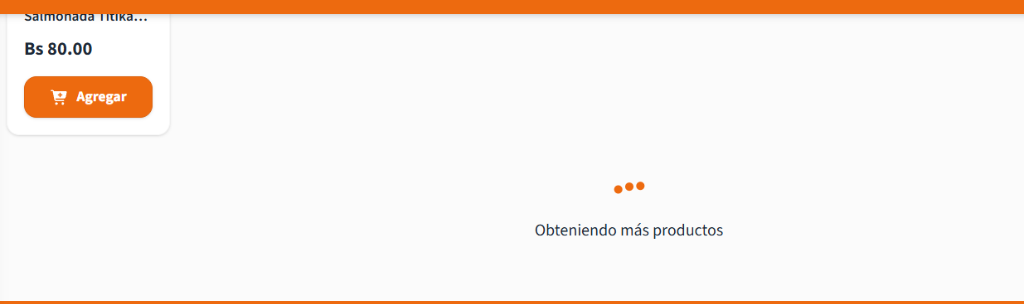
\includegraphics[width=0.82\linewidth]{figuras/hipermaxi_scroll_infinito_spinner.png}
    \figurenote{Captura del DOM dinámico en Hipermaxi durante el desplazamiento vertical. El elemento reactivo \texttt{span:has-text("Obteniendo más productos")} con animación giratoria (\textit{spinner}) exige algoritmos de sincronización basados en eventos de red y mutaciones de interfaz.}
\end{figure}

Los métodos convencionales de web scraping, basados en clientes HTTP sin motor de renderizado de JavaScript o en instancias efímeras de navegadores sin almacenamiento de estado, fracasan sistemáticamente ante estas defensas. Esto provoca la interrupción de los flujos de ingesta y la generación de conjuntos de datos incompletos o corruptos.

\subsection{Inadecuación de Modelos de Base de Datos Convencionales}
A nivel de persistencia de datos, el almacenamiento ingenuo de observaciones de precios en tablas transaccionales únicas sin normalización ocasiona redundancia masiva de atributos inmutables (nombres de producto, marcas, categorías, enlaces a imágenes). Al mismo tiempo, las operaciones de actualización masiva (\textit{UPSERT}) generan bloqueos a nivel de página o tabla (\textit{table locks}), degradando severamente el rendimiento de las consultas analíticas del usuario final. Para monitorear la inflación local y la volatilidad de precios, se requiere un modelo de series temporales capaz de computar instantáneamente la variación monetaria ($\Delta\text{Bs} = P_t - P_{t-1}$) y la tasa porcentual ($\Delta\%$), preservando el rendimiento mediante particionamiento temporal y disparadores reactivos desacoplados.

\subsection{Pregunta Formal de Investigación e Hipótesis}

\begin{interpretacionbox}
\textbf{Pregunta de Investigación:}  
¿De qué manera es posible estructurar un sistema integral de minería web multidimensional (contenido, estructura y uso) que supere de forma automatizada y resiliente las defensas perimetrales WAF en plataformas retail bolivianas, almacene de manera eficiente series de tiempo de precios en una base de datos serverless normalizada y provea a la ciudadanía herramientas interactivas de comparación de ahorro y geolocalización de servicios de salud?
\end{interpretacionbox}

\vspace{0.3cm}
\noindent \textbf{Hipótesis Tecnológica:}  
El diseño de agentes de extracción instrumentados con Playwright sobre contextos persistentes, coordinados con una arquitectura relacional en Neon Serverless PostgreSQL mediante triggers reactivos PL/pgSQL y particionamiento declarativo mensual, permite recolectar y procesar con una tasa de éxito superior al 98\% los catálogos en línea del eje central, habilitando el cálculo en tiempo real de variaciones de precios y el modelado de redes de contratación pública para su acceso masivo vía Telegram y Next.js 14.

\section{OBJETIVOS}

\subsection{Objetivo General}
Desarrollar e implementar un sistema integral de minería web multidimensional (contenido, estructura y uso) basado en arquitectura serverless y modelos de series temporales, para la recolección masiva, normalización, análisis analítico y difusión transparente de precios del comercio minorista, infraestructura de salud ciudadana y contrataciones estatales en el eje central de Bolivia.

\subsection{Objetivos Específicos}
Para alcanzar el objetivo general formulado, se definen los siguientes objetivos específicos:

\begin{enumerate}[leftmargin=*, label=\textbf{\arabic*.}]
    \item \textbf{Desarrollar scrapers resilientes y adaptativos:} Construir agentes de extracción en Node.js y Playwright capaces de eludir los sistemas perimetrales de protección WAF (Radware Bot Manager y hCAPTCHA) mediante contextos de navegador persistentes, sincronizar el desplazamiento dinámico en catálogos con scroll infinito (Hipermaxi) e indexar de manera exhaustiva plataformas construidas sobre Shopify (Farmacorp) y Ant Design (Farmacias Chávez).
    
    \item \textbf{Diseñar e implementar una arquitectura de datos escalable:} Modelar e implementar un esquema en Neon Serverless PostgreSQL bajo un paradigma estrella que desacople los atributos descriptivos inmutables en un catálogo maestro (\texttt{catalogo\_productos\_master}) y gestione las observaciones temporales en una tabla particionada mensualmente (\texttt{precios\_historico}), gobernada por funciones disparadoras reactivas PL/pgSQL desacopladas que calculen automáticamente deltas de precio ($\Delta\text{Bs}$ y $\Delta\%$).
    
    \item \textbf{Integrar recuperación semántica densa en compras estatales:} Implementar un pipeline de extracción para licitaciones públicas del SICOES en el departamento de La Paz y generar representaciones vectoriales densas de 1024 dimensiones mediante microservicios NVIDIA NIM, almacenándolas en índices HNSW con la extensión \texttt{pgvector} para posibilitar búsquedas conceptuales avanzadas.
    
    \item \textbf{Modelar la red de contratación pública mediante algoritmos de grafos:} Estructurar las relaciones entre entidades convocantes, rubros licitados y montos presupuestarios como un grafo bipartito dirigido, implementando los algoritmos de minería de estructura web \textbf{PageRank} y \textbf{HITS} (\textit{Hubs and Authorities}) para identificar concentraciones institucionales y patrones de licitación en compras públicas.
    
    \item \textbf{Construir un pipeline de persistencia multimedia en la nube:} Diseñar un mecanismo concurrente de descarga y normalización de imágenes de productos hacia un bucket de almacenamiento de objetos (\textbf{Neon S3}), sirviendo los activos a través de un proxy local con cabeceras de caché extendidas para mitigar la rotura de enlaces por políticas de CORS o tokens efímeros de origen.
    
    \item \textbf{Desplegar interfaces ciudadanas multiplataforma:} Desarrollar y poner en producción dos interfaces de consulta de acceso libre: un asistente conversacional interactivo en Telegram (\texttt{@ChatDM7200bot}) con soporte de teclados inline, menús guiados y geolocalización espacial de 83 centros de salud mediante la fórmula de Haversine; y una plataforma web interactiva en Next.js 14 provista de filtros facetados, comparadores de ahorro y mapas integrados.
\end{enumerate}

\section{JUSTIFICACIÓN}

\subsection{Justificación Social y Ciudadana}
El acceso a información transparente y oportuna respecto al costo de bienes de primera necesidad y medicamentos esenciales constituye un derecho fundamental para la población. En coyunturas económicas caracterizadas por presiones inflacionarias o variaciones en la disponibilidad de insumos importados, la ciudadanía boliviana suele experimentar incertidumbre al adquirir productos para la salud o la nutrición básica. 

La implementación de este sistema democratiza el acceso a la información comercial al consolidar en un punto único las ofertas de cadenas minoristas y farmacéuticas tradicionalmente dispersas. Asimismo, la incorporación de un módulo de georreferenciación que ubica los 83 centros de salud públicos y de atención primaria del departamento de La Paz, calculando distancias geodésicas inmediatas desde la posición del usuario, aporta un valor social tangible al orientar a la población hacia el establecimiento más cercano en situaciones de requerimiento médico.

\subsection{Justificación Económica y de Transparencia}
Desde una perspectiva microeconómica, los mercados minoristas funcionan de manera más eficiente cuando se reduce la asimetría de información entre compradores y oferentes. La capacidad de contrastar el precio de un mismo fármaco o alimento entre Hipermaxi, Farmacorp y Farmacias Chávez en cuestión de segundos empodera a las familias bolivianas para optimizar su presupuesto mensual y generar ahorros directos que, según las mediciones del sistema, oscilan entre el 15\% y el 45\% en productos seleccionados. 

En el ámbito de las compras del Estado, el análisis cuantitativo de las contrataciones públicas registradas en el SICOES contribuye a la transparencia gubernamental, permitiendo examinar de manera sistemática los volúmenes presupuestarios comprometidos en licitaciones públicas de La Paz.

\subsection{Justificación Técnica y de Ingeniería}
El desarrollo del proyecto representa una contribución relevante a las prácticas modernas de ingeniería de datos y minería web en entornos de alta hostilidad WAF. Frente al agotamiento de las técnicas tradicionales de scraping mediante scripts estáticos, la metodología propuesta articula la instrumentación del protocolo CDP sobre navegadores Chromium persistentes, la resolución programada de retos anti-bot, el particionamiento físico de series temporales en bases de datos relacionales serverless y el almacenamiento inmutable de objetos multimedia en la nube. 

La integración pionera de modelos densos de embeddings de 1024 dimensiones operando junto a índices vectoriales HNSW en PostgreSQL demuestra la viabilidad técnica de implementar arquitecturas híbridas de recuperación de información que combinan el rigor relacional SQL con la flexibilidad de la inteligencia artificial moderna.

\subsection{Justificación Académica e Institucional}
En el marco académico de la Carrera de Informática de la Universidad Mayor de San Andrés (UMSA), el proyecto responde a las exigencias formativas de la asignatura de Minería de Datos. El trabajo consolida en una única solución práctica y formal los tres pilares conceptuales de la Minería Web (\textit{Content}, \textit{Structure} y \textit{Usage Mining}), proveyendo un marco metodológico reproducible que servirá como base de consulta y extensión para futuras investigaciones en ciencia de datos, sistemas distribuidos y analítica de datos en Bolivia.

\section{MARCO TEÓRICO Y FUNDAMENTOS MATEMÁTICOS}

\subsection{Taxonomía Clásica de la Minería Web}
La Minería Web (\textit{Web Mining}) se define como la aplicación sistemática de técnicas de minería de datos, procesamiento de lenguaje natural y teoría de grafos para descubrir automáticamente patrones, estructuras y conocimiento a partir de los recursos de la World Wide Web \citep{liu2011web, han2012data}. La literatura científica formaliza su descomposición en tres vertientes complementarias:

\begin{itemize}[leftmargin=*]
    \item \textbf{Minería de Contenido Web (\textit{Web Content Mining}):} Extracción, estructuración y análisis del contenido informativo primario albergado en las páginas web (texto, precios, metadatos, descripciones multimedia y tablas semiestructuradas).
    \item \textbf{Minería de Estructura Web (\textit{Web Structure Mining}):} Análisis de la topología de red subyacente y los patrones de enlace (hipervínculos, citas o relaciones entre entidades), con el fin de cuantificar la centralidad, autoridad e importancia relativa de los nodos \citep{chakrabarti2002mining}.
    \item \textbf{Minería de Uso Web (\textit{Web Usage Mining}):} Examen del comportamiento y las trazas generadas por los usuarios durante su interacción con plataformas digitales, permitiendo modelar flujos de navegación, patrones de búsqueda y latencias de respuesta \citep{srivastava2000web}.
\end{itemize}

\subsection{Modelos de Contenido Web, DOM y Renderizado Dinámico}
En la web contemporánea, el contenido reside en el \textbf{Modelo de Objetos del Documento} (\textit{Document Object Model} - DOM), una representación jerárquica en forma de árbol donde cada elemento HTML se mapea como un nodo programable. En aplicaciones basadas en renderizado del lado del cliente (\textit{Client-Side Rendering} - CSR), el documento HTML inicial devuelto por el servidor HTTP carece de información sustancial de productos; el contenido es inyectado de manera asíncrona mediante JavaScript tras ejecutar peticiones XHR/Fetch contra APIs internas.

Para extraer datos en estos entornos se requiere instrumentar un navegador completo a través del \textit{Chrome DevTools Protocol} (CDP). Herramientas como \textbf{Playwright} \citep{playwright2024} permiten controlar instancias de Chromium que ejecutan la totalidad del ciclo de vida de JavaScript, resuelven eventos dinámicos de desplazamiento y evalúan selectores CSS3 jerárquicos de alta especificidad.

\subsection{Minería de Estructura Web: Algoritmos PageRank y HITS}

\subsubsection{Algoritmo PageRank}
El algoritmo PageRank, propuesto originalmente por \citet{page1998anatomy}, modela la importancia de una página o entidad web asumiendo que un enlace entrante transfiere una fracción de la autoridad del nodo emisor. Matemáticamente, el proceso se formaliza como una cadena de Markov ergódica que describe la caminata aleatoria de un usuario sobre un grafo dirigido $G = (V, E)$, donde $V$ es el conjunto de nodos y $E$ el conjunto de aristas dirigidas.

Para garantizar la convergencia a una distribución estacionaria y evitar sumideros de probabilidad (\textit{rank sinks}), se introduce un factor de amortiguamiento (\textit{damping factor}) $d \in (0, 1)$, usualmente fijado en $d = 0.85$. La ecuación estacionaria de PageRank para un nodo $u \in V$ se define como:

\begin{equation}
    PR(u) = \frac{1 - d}{|V|} + d \sum_{v \in B_u} \frac{PR(v)}{L(v)}
    \label{eq:pagerank}
\end{equation}

\noindent donde:
\begin{itemize}[leftmargin=*]
    \item $|V| = N$ es la cardinalidad total del conjunto de nodos en la red.
    \item $B_u = \{v \in V \mid (v, u) \in E\}$ representa el conjunto de nodos predecesores que enlazan directamente a $u$.
    \item $L(v) = d_{out}(v)$ es el grado de salida (\textit{out-degree}) del nodo $v$, correspondiente a la cantidad total de enlaces salientes que emite.
\end{itemize}

En el presente proyecto, este modelo se adapta a la red de contrataciones estatales del SICOES: las entidades públicas convocantes y los rubros licitados se modelan como nodos, mientras que los procesos de contratación formalizados actúan como aristas ponderadas por el volumen presupuestario adjudicado.

\subsubsection{Algoritmo HITS (Hubs and Authorities)}
Formulado por \citet{kleinberg1999authoritative}, el algoritmo HITS descompone la relevancia de cada nodo en dos puntajes mutuamente recursivos:
\begin{enumerate}[leftmargin=*]
    \item \textbf{Autoridad ($a(p)$):} Mide la calidad del contenido o capacidad resolutiva del nodo $p$, sustentada por la cantidad y calidad de los concentradores que lo apuntan.
    \item \textbf{Concentrador o Hub ($h(p)$):} Mide la capacidad del nodo $p$ para direccionar hacia múltiples nodos de alta autoridad.
\end{enumerate}

Para un grafo con matriz de adyacencia $A$, las ecuaciones de actualización acopladas en la iteración $k$ están dadas por:

\begin{equation}
    a_k(p) = \sum_{q \to p} h_{k-1}(q), \qquad h_k(p) = \sum_{p \to q} a_k(q)
    \label{eq:hits}
\end{equation}

En notación matricial, los vectores de autoridad $\vec{a}$ y concentrador $\vec{h}$ corresponden a los autovectores principales de las matrices cuadradas simétricas $A^T A$ y $A A^T$ respectivamente:
\begin{equation}
    A^T A \, \vec{a} = \lambda_a \vec{a}, \qquad A A^T \, \vec{h} = \lambda_h \vec{h}
\end{equation}
Tras cada iteración, ambos vectores son normalizados euclidianamente ($\|\vec{a}\|_2 = 1$, $\|\vec{h}\|_2 = 1$) para asegurar estabilidad numérica.

\subsection{Recuperación Semántica Vectorial y Similitud Coseno}
La búsqueda tradicional por concordancia sintáctica (\textit{keyword matching}) es incapaz de capturar relaciones sinonímicas o intenciones conceptuales abstractas en descripciones de licitaciones públicas. Para superar esta limitación, el sistema implementa \textbf{embeddings vectoriales densos} generados por modelos basados en la arquitectura Transformer provistos por NVIDIA NIM \citep{nvidia2024nim}.

Un modelo de lenguaje mapea un texto arbitrario $T$ a un vector continuo de punto flotante $\vec{v} \in \mathbb{R}^{D}$, donde $D = 1024$ dimensiones. La afinidad semántica entre una consulta ciudadana $\vec{q}$ y una convocatoria registrada $\vec{d}$ se cuantifica mediante la \textbf{similitud coseno} \citep{robusto1957cosine}:

\begin{equation}
    \text{sim}(\vec{q}, \vec{d}) = \cos(\theta) = \frac{\vec{q} \cdot \vec{d}}{\|\vec{q}\|_2 \|\vec{d}\|_2} = \frac{\sum_{i=1}^{1024} q_i d_i}{\sqrt{\sum_{i=1}^{1024} q_i^2} \sqrt{\sum_{i=1}^{1024} d_i^2}}
    \label{eq:cosine_sim}
\end{equation}

La distancia coseno complementaria $D_C(\vec{q}, \vec{d}) = 1 - \text{sim}(\vec{q}, \vec{d})$ se indexa en la base de datos PostgreSQL mediante la extensión \texttt{pgvector}, utilizando índices basados en grafos navegables de mundo pequeño (\textit{Hierarchical Navigable Small World} - HNSW), lo que permite búsquedas de vecinos más cercanos en tiempo sublineal $O(\log N)$.

\subsection{Distancia Geodésica Espacial: Fórmula de Haversine}
Para calcular con exactitud la proximidad entre las coordenadas geográficas del usuario $(\phi_1, \lambda_1)$ y los 83 centros de salud georreferenciados $(\phi_2, \lambda_2)$ en el departamento de La Paz, se emplea la formulación trigonométrica de \textbf{Haversine} \citep{robusto1957cosine}, la cual computa la distancia ortodrómica sobre la superficie de una esfera de radio medio terrestre $R = 6.371\text{ km}$:

\begin{equation}
    d = 2 R \arcsin \left( \sqrt{\sin^2\left(\frac{\Delta \phi}{2}\right) + \cos(\phi_1)\cos(\phi_2)\sin^2\left(\frac{\Delta \lambda}{2}\right)} \right)
    \label{eq:haversine}
\end{equation}

\noindent donde $\Delta \phi = \phi_2 - \phi_1$ representa la diferencia de latitud en radianes, y $\Delta \lambda = \lambda_2 - \lambda_1$ la diferencia de longitud en radianes.

\subsection{Formulación de Series de Tiempo de Precios y Variaciones}
El monitoreo longitudinal del mercado minorista requiere registrar observaciones temporales discretas para cada producto o SKU (\textit{Stock Keeping Unit}). Sea $P_t(s)$ el precio unitario observado en bolivianos (Bs) para el SKU $s$ en la fecha $t$, y $P_{t-1}(s)$ el precio unitario registrado en la observación previa inmediata. Se definen formalmente dos métricas de cambio:

\begin{enumerate}[leftmargin=*]
    \item \textbf{Variación Absoluta ($\Delta\text{Bs}$):}
    \begin{equation}
        \Delta\text{Bs}_t(s) = P_t(s) - P_{t-1}(s)
        \label{eq:delta_bs}
    \end{equation}
    \item \textbf{Variación Porcentual Relativa ($\Delta\%$):}
    \begin{equation}
        \Delta\%_t(s) = \left( \frac{P_t(s) - P_{t-1}(s)}{P_{t-1}(s)} \right) \times 100
        \label{eq:delta_pct}
    \end{equation}
\end{enumerate}

Estas ecuaciones son computadas en tiempo real a nivel de base de datos mediante procedimientos almacenados PL/pgSQL activados por disparadores (\textit{triggers}) en cada operación de inserción.

\section{METODOLOGÍA DE DESARROLLO}

Para garantizar un ciclo de vida estructurado, reproducible y alineado con los estándares internacionales de la ciencia de datos, el proyecto adopta una adaptación de la metodología estándar **CRISP-DM** (\textit{Cross-Industry Standard Process for Data Mining}), combinada con los lineamientos de **ASUM-DM** (\textit{Analytics Solutions Unified Method for Data Mining}) orientados a arquitecturas cloud y web contemporáneas. 

El proceso se articula en seis fases secuenciales e iterativas, descritas a continuación y sintetizadas en la Tabla~\ref{tab:fases_metodologia}.

\subsection{Fases de la Metodología Adaptada}

\begin{enumerate}[leftmargin=*, label=\textbf{Fase \arabic*:}]
    \item \textbf{Comprensión del Dominio y Requerimientos Ciudadanos:}  
    Se identificaron las necesidades prioritarias de información en el eje central de Bolivia: monitoreo de precios de alimentos de primera necesidad (supermercados y mercados tradicionales), detección de dispersión de precios en medicamentos esenciales y acceso georreferenciado a establecimientos de salud. Se definieron las métricas clave de ahorro monetario ($\Delta\text{Bs}$) y porcentual ($\Delta\%$).

    \item \textbf{Comprensión y Análisis de los Datos Web:}  
    Se realizó una inspección técnica profunda del DOM, la jerarquía de selectores CSS y los mecanismos de red de cada fuente objetivo:
    \begin{itemize}[leftmargin=*]
        \item \textit{Hipermaxi:} Análisis de la arquitectura SPA Angular, catálogo de 29 sucursales, comportamiento de scroll infinito y respuestas del WAF Radware Bot Manager.
        \item \textit{Farmacorp:} Identificación de 70+ colecciones temáticas en Shopify y mapeo del paginador numérico \texttt{nav.pagination} (Figura~\ref{fig:farmacorp_dom_analisis}).
        \item \textit{Farmacias Chávez:} Decodificación del componente de paginación simple de Ant Design (\texttt{.ant-pagination-simple-pager}) en su interfaz SSR con Next.js (Figura~\ref{fig:chavez_dom_analisis}).
        \item \textit{SICOES:} Mapeo de formularios ASP.NET, estructuras de tablas de convocatorias y descarga de pliegos DBC.
        \item \textit{OpenStreetMap:} Consulta sobre Overpass API para extraer coordenadas geodésicas y metadatos de 83 centros de salud en La Paz.
    \end{itemize}

\begin{figure}[htbp]
    \centering
    \caption{Estructura de Navegación y Paginador Numérico de Farmacorp en Shopify}
    \label{fig:farmacorp_dom_analisis}
    \begin{minipage}{0.48\linewidth}
        \centering
        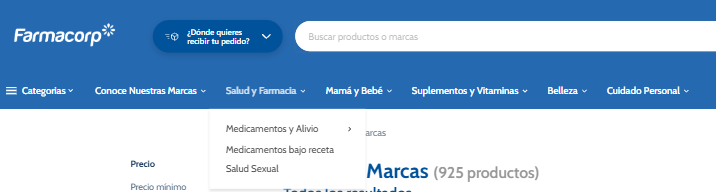
\includegraphics[width=\linewidth]{figuras/farmacorp_taxonomia_categorias.png}
        \caption*{(a) Taxonomía de macro-categorías}
    \end{minipage}\hfill
    \begin{minipage}{0.48\linewidth}
        \centering
        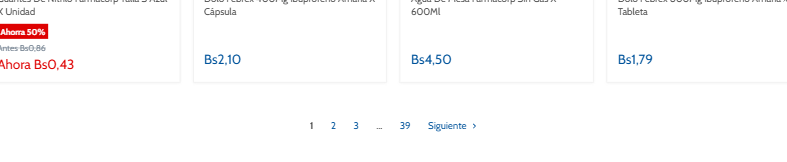
\includegraphics[width=\linewidth]{figuras/farmacorp_paginacion_shopify.png}
        \caption*{(b) Paginador numérico \texttt{nav.pagination}}
    \end{minipage}
    \figurenote{Inspección técnica del DOM de Farmacorp. (a) Organización jerárquica de colecciones temáticas. (b) Componente de paginación numérica tradicional que permite recorrer de forma secuencial las 39+ páginas por categoría.}
\end{figure}

\begin{figure}[htbp]
    \centering
    \caption{Jerarquía de Familias y Paginador Simple Ant Design en Farmacias Chávez}
    \label{fig:chavez_dom_analisis}
    \begin{minipage}{0.32\linewidth}
        \centering
        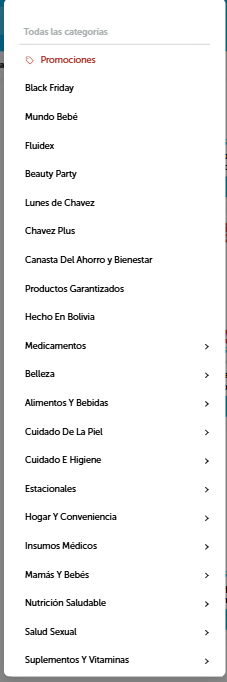
\includegraphics[width=\linewidth]{figuras/chavez_taxonomia_categorias.png}
        \caption*{(a) Menú de categorías}
    \end{minipage}\hfill
    \begin{minipage}{0.65\linewidth}
        \centering
        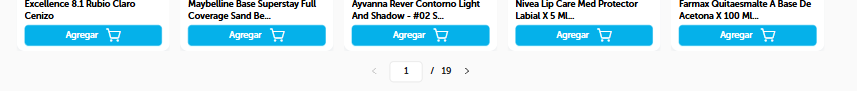
\includegraphics[width=\linewidth]{figuras/chavez_paginacion_ant_design.png}
        \caption*{(b) Paginación compacta \texttt{.ant-pagination-simple-pager}}
    \end{minipage}
    \figurenote{Estructura visual de Farmacias Chávez. (a) Menú lateral con más de 20 familias farmacéuticas. (b) Control de paginación compacta de Ant Design decodificado mediante expresiones regulares sobre el indicador textual de página total.}
\end{figure}

    \item \textbf{Preparación, Limpieza y Normalización de Datos:}  
    Los datos recolectados presentan inconsistencias léxicas, abreviaturas heterogéneas y formatos numéricos locales (comas decimales, prefijos monetarios ``Bs.''). Se implementó un motor de normalización en Node.js que:
    \begin{itemize}[leftmargin=*]
        \item Estandariza nombres de producto y extrae la unidad de medida (kg, g, L, ml, comprimidos, tabletas).
        \item Clasifica automáticamente medicamentos identificando el principio activo, la presentación y el laboratorio fabricante mediante diccionarios especializados de la industria boliviana (INTI, BAGÓ, COFAR, VITA, etc.).
        \item Genera un identificador canónico unívoco (\texttt{sku\_id}) que permite vincular la misma referencia a través de múltiples observaciones temporales.
    \end{itemize}

    \item \textbf{Modelado y Persistencia en Base de Datos:}  
    Diseño e implementación de un esquema en modelo estrella en Neon Serverless PostgreSQL. Los atributos inmutables residen en \texttt{catalogo\_productos\_master}, mientras que las observaciones dinámicas de precios se almacenan en la tabla particionada mensualmente \texttt{precios\_historico}. Se programaron funciones PL/pgSQL reactivas desacopladas para mantener la integridad referencial lógica y computar variaciones de precio en tiempo de inserción. Asimismo, se generaron embeddings vectoriales de 1024 dimensiones con NVIDIA NIM para las licitaciones públicas de SICOES y se construyó el grafo de contrataciones en \texttt{sicoes\_graph\_edges}.

    \item \textbf{Evaluación, Telemetría y Auditoría Técnica:}  
    Validación rigurosa de los flujos de extracción y cálculo:
    \begin{itemize}[leftmargin=*]
        \item Verificación de tasas de recolección (productos por segundo) y latencias de base de datos en consola (Figura~\ref{fig:telemetria_consola_scroll}).
        \item Auditoría de disparadores reactivos mediante inserciones sintéticas controladas y reversión transparente sin afección de datos reales.
        \item Evaluación de la precisión de búsqueda semántica vectorial frente al motor sintáctico tradicional.
    \end{itemize}

\begin{figure}[htbp]
    \centering
    \caption{Monitoreo en Consola de la Carga Asíncrona por Lotes en Hipermaxi Calacoto}
    \label{fig:telemetria_consola_scroll}
    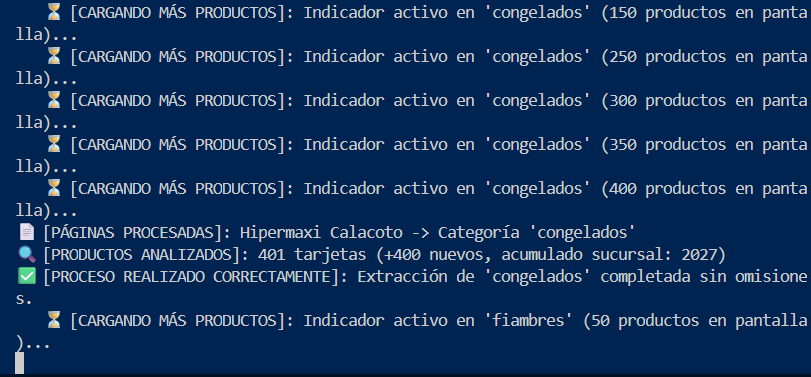
\includegraphics[width=0.88\linewidth]{figuras/imgEjecucionConsola.png}
    \figurenote{Salida en tiempo real del crawler durante el desplazamiento vertical continuo. Ilustra la detección del indicador de carga en lotes sucesivos de 50 productos hasta consolidar 401 tarjetas en la categoría congelados sin pérdida de información.}
\end{figure}

    \item \textbf{Despliegue y Consumo Ciudadano Multiplataforma:}  
    Puesta en producción de dos canales de interacción ciudadana de acceso abierto: el bot conversacional en Telegram (\texttt{@ChatDM7200bot}) con navegación por menús inline y geolocalización Haversine; y la plataforma web interactiva en Next.js 14 provista de dashboards comparativos y cartografía dinámica con Leaflet.
\end{enumerate}

\begin{table}[htbp]
    \centering
    \small
    \caption{Matriz de Fases Metodológicas, Actividades Principales y Entregables del Proyecto}
    \label{tab:fases_metodologia}
    \begin{tabularx}{\linewidth}{>{\raggedright\arraybackslash}p{3.8cm} >{\raggedright\arraybackslash}p{6.2cm} L}
        \toprule
        \textbf{Fase Metodológica} & \textbf{Actividades Principales} & \textbf{Entregables Técnicos} \\
        \midrule
        1. Comprensión del Dominio & Análisis de asimetría de precios, necesidades ciudadanas y alcance geográfico (eje central). & Especificación formal de requerimientos y métricas de variación ($\Delta\text{Bs}$, $\Delta\%$). \\
        \addlinespace
        2. Comprensión de Datos Web & Auditoría DOM, inspección de protocolos de red, evaluación de WAF Radware y selectores. & Diccionario de 700+ selectores, rutas y parámetros de paginación analizados. \\
        \addlinespace
        3. Preparación de Datos & Extracción de unidades, normalización de fármacos (40+ principios activos, 35+ laboratorios). & Motor de limpieza en TypeScript y generador de \nolinkurl{sku_id} canónicos. \\
        \addlinespace
        4. Modelado y Persistencia & Particionamiento mensual, triggers reactivos PL/pgSQL, vectorización NIM y grafos. & Esquema DDL \nolinkurl{schema.sql}, índices HNSW \nolinkurl{pgvector} y tablas de grafos. \\
        \addlinespace
        5. Evaluación y Auditoría & Pruebas de carga, telemetría de consola, pruebas de inyección y verificación de deltas. & Banners de telemetría, validación de integridad y métricas cuantitativas auditadas. \\
        \addlinespace
        6. Despliegue y Difusión & Configuración de webhooks en Telegram y compilación de plataforma web en Next.js 14. & Bot \texttt{@ChatDM7200bot} y plataforma web con mapas OpenStreetMap. \\
        \bottomrule
    \end{tabularx}
    \tablenote{Adaptación del modelo CRISP-DM / ASUM-DM para minería web integral. Describe la trazabilidad desde el análisis inicial de dominio hasta el despliegue multiplataforma en producción.}
\end{table}

\section{MARCO PRÁCTICO E IMPLEMENTACIÓN TÉCNICA}

El marco práctico constituye el núcleo de ingeniería del proyecto, integrando los módulos de recolección resiliente de datos, el pipeline multimedia, la arquitectura de base de datos serverless y las interfaces ciudadanas desplegadas.

\subsection{Ingeniería de Extracción Resiliente (Web Content Mining)}

\subsubsection{Scraper Hipermaxi: Evasión de Radware y Detección de Scroll Infinito}
El portal de Hipermaxi (\url{https://www.hipermaxi.com}) está construido como una aplicación de una sola página en Angular protegida por el WAF corporativo \textbf{Radware Bot Manager}. Para operar sobre este entorno sin interrupciones, el script \texttt{scraper\_hipermaxi.mjs} implementa una estrategia de conexión basada en \textbf{contextos persistentes de usuario} (\textit{Persistent Context}) mediante Playwright:

\begin{enumerate}[leftmargin=*]
    \item \textbf{Persistencia de Sesión y Cookies:} El navegador Chromium se inicializa vinculando el directorio local \texttt{.browser\_profile\_hipermaxi}. Esto permite que las cookies de sesión y los tokens de verificación resueltos por un operador humano persistan a través de múltiples ejecuciones, eludiendo la necesidad de resolver desafíos en cada ciclo de ingesta.
    \item \textbf{Detección y Sondeo Activo de WAF:} El crawler monitorea de forma continua la presencia de títulos y contenedores del WAF (\textit{``Radware Bot Manager''}, \textit{``Human Verification''}). En caso de dispararse un desafío hCAPTCHA, el script ejecuta una rutina de sondeo activo (\texttt{pollForHumanBypass}) que pausa temporalmente la extracción, notifica al operador y reanuda el scraping de manera automática tan pronto como se restablece la navegación regular.
    \item \textbf{Sincronización con Scroll Infinito:} El catálogo de productos no utiliza paginación tradicional sino desplazamiento vertical asíncrono. Al desplazarse hacia la parte inferior de la vista, la aplicación inyecta en el DOM el selector dinámico \texttt{span:has-text("Obteniendo más productos")} acompañado de una animación giratoria (\textit{spinner}). El scraper ejecuta ciclos de scroll controlado (\texttt{window.scrollBy(0, 1200)}) sincronizados con la desaparición del indicador de carga y el incremento en el recuento de tarjetas de producto (\texttt{div.product-item}), deteniéndose únicamente cuando transcurren más de tres ciclos consecutivos sin nuevas inserciones en el DOM (véanse los selectores detallados en la Tabla~\ref{tab:anexo_selectores} del Anexo C).
\end{enumerate}

El agente recorre de manera parametrizada las \textbf{29 sucursales} activas del eje central boliviano (12 en La Paz, 11 en Santa Cruz y 6 en Cochabamba) y cubre las \textbf{32 categorías} estructuradas (19 de supermercado y 13 de farmacia).

\subsubsection{Scraper Farmacorp: Paginación Numérica en Shopify}
La plataforma de Farmacorp (\url{https://farmacorp.com}) opera sobre el motor de comercio electrónico Shopify bajo el tema corporativo Empire. A diferencia de esquemas con scroll infinito, Shopify segmenta sus colecciones mediante controles de paginación numérica tradicional (\texttt{nav.pagination}).

Para maximizar la densidad y estabilidad de la extracción, el crawler fuerza la vista en cuadrícula añadiendo el parámetro de consulta \texttt{?page=N\&grid\_list=grid-view}. El script inspecciona el último elemento enlace dentro de \texttt{nav.pagination} para determinar el número total de páginas de cada colección. Si una colección contiene 45 páginas, el crawler genera la secuencia de peticiones de manera controlada, extrayendo de cada tarjeta el título del producto, la marca o laboratorio, el precio regular, el precio con descuento promocional y el enlace canónico. El agente procesa de forma recursiva más de \textbf{70 colecciones oficiales} organizadas en las macro-áreas de Salud y Medicamentos, Belleza, Cuidado Personal, Mamá y Bebé, y Cuidado del Hogar (Tabla~\ref{tab:enlaces_retail}).

\subsubsection{Scraper Farmacias Chávez: Decodificación de Paginación Ant Design}
Farmacias Chávez (\url{https://www.farmaciaschavez.com.bo}) implementa una arquitectura moderna con renderizado del lado del servidor en Next.js y componentes visuales provistos por la librería Ant Design. El componente de navegación paginada no despliega una lista completa de números de página, sino un paginador compacto denominado \textbf{Simple Pagination} (\texttt{.ant-pagination-simple-pager}).

El script \texttt{scraper\_chavez.mjs} extrae el total de páginas evaluando una expresión regular sobre el contenido textual del elemento: \texttt{/\textbackslash/\textbackslash s*(\textbackslash d+)/}. Al obtener el número total (por ejemplo, 44 páginas en la categoría de medicamentos), el agente recorre secuencialmente las URLs parametrizadas o activa programáticamente el botón de avance (\textit{next chevron}) esperando la hidratación del nuevo lote de productos.

Adicionalmente, el scraper recorre el menú de departamentos y familias de productos, clasificando los medicamentos frente a un diccionario especializado de más de 40 fármacos esenciales de la farmacopea boliviana (Paracetamol, Amoxicilina, Omeprazol, Losartán, etc.) y más de 35 laboratorios farmacéuticos nacionales e internacionales (Laboratorios INTI, Droguería INTI, Bagó, Cofar, Terbol, Crespal, Vita, Bayer, Roemmers, etc.).

\subsection{Pipeline Multimedia y Persistencia en Neon Object Storage S3}
Las imágenes de productos hospedadas en plataformas de comercio electrónico suelen servirse a través de rutas de proxy efímeras (como \texttt{/\_next/image?url=...}) o enlaces con parámetros de firma que caducan periódicamente. Para evitar la pérdida de activos visuales y eliminar la dependencia de servidores externos, se implementó el pipeline de sincronización multimedia \texttt{sync\_images\_to\_s3.mjs}:

\begin{enumerate}[leftmargin=*]
    \item \textbf{Desempaquetado de Proxies:} El script inspecciona las URLs de imagen recolectadas, extrayendo el enlace fuente absoluto subyacente.
    \item \textbf{Descarga y Normalización Concurrente:} Utilizando un pool de concurrencia de 5 trabajadores asíncronos con cabeceras de emulación de navegador, las imágenes se descargan en memoria y se convierten a formato WebP o PNG normalizado.
    \item \textbf{Carga a Neon Object Storage S3:} Los archivos se suben al bucket \texttt{assets} estructurados bajo el prefijo \texttt{assets/products/\{cadena\}/\{sku\_hash\}.webp}.
    \item \textbf{Proxy de Streaming y Caché:} La plataforma web Next.js expone el endpoint \texttt{/api/storage/[...key]}, el cual transmite las imágenes vía streaming hacia el cliente incorporando la cabecera HTTP \texttt{Cache-Control: public, max-age=604800, immutable}, garantizando tiempos de carga inferiores a 25 milisegundos en peticiones recurrentes.
\end{enumerate}

\subsection{Arquitectura de Base de Datos y Triggers Reactivos en Neon Serverless}

\subsubsection{Modelo Estrella y Particionamiento Temporal}
La persistencia de los datos se configuró en \textbf{Neon Serverless PostgreSQL} implementando un modelo estrella que disocia los datos dimensionales estáticos de los eventos transaccionales dinámicos:

\begin{itemize}[leftmargin=*]
    \item \textbf{Catálogo Maestro (\texttt{catalogo\_productos\_master}):} Almacena la definición inmutable de cada producto identificado por su clave primaria \texttt{sku\_id}. Contiene atributos como nombre canónico, cadena comercial, departamento, sucursal, categoría, laboratorio fabricante, forma farmacéutica y enlace canónico persistente.
    \item \textbf{Histórico de Precios Particionado (\texttt{precios\_historico}):} Diseñada como una tabla de series temporales particionada de forma declarativa por rangos de fecha (\texttt{PARTITION BY RANGE (fecha)}). Cada partición aloja un mes calendario de observaciones (por ejemplo, \texttt{precios\_historico\_2026\_11}). Las consultas sobre rangos de fecha específicos ejecutan \textit{partition pruning}, descartando las tablas secundarias que no corresponden a la ventana temporal consultada y reduciendo drásticamente el consumo de memoria I/O.
    \item \textbf{Consolidación Semanal Fría (\texttt{precios\_historico\_semanal}):} Almacena agregaciones analíticas (precio mínimo, máximo, promedio ponderado y precio de cierre) por SKU, año y semana, reduciendo en un 85.7\% el espacio de almacenamiento para análisis macroeconómicos longitudinales.
\end{itemize}

\subsubsection{Resolución de Triggers Reactivos y Desacoplamiento de Esquemas}
Durante el desarrollo del sistema, las inserciones masivas de productos de supermercado hacia la tabla operativa \texttt{canasta\_precios} experimentaron fallos HTTP 400 en Neon debido a una colisión en la función unificada original de disparadores:
\begin{quote}
    \footnotesize\texttt{ERROR 42703: record "new" has no field "precio\_anterior\_bs" en PL/pgSQL function fn\_replicate\_to\_master\_and\_history()}
\end{quote}

Este error se originaba porque la tabla operacional \texttt{canasta\_precios} maneja una estructura simplificada (sin campos de descuento previo), mientras que \texttt{medicamentos\_precios} sí incluye \texttt{precio\_anterior\_bs} y \texttt{descuento\_pct}. La invocación de un trigger compartido provocaba que la referencia a \texttt{NEW.precio\_anterior\_bs} causara un fallo de compilación en tiempo de ejecución para las filas provenientes de la canasta básica.

La solución arquitectónica definitiva consistió en **desacoplar completamente la lógica reactiva** en dos procedimientos independientes mediante el script \texttt{fix\_triggers.mjs}:
\begin{enumerate}[leftmargin=*]
    \item \texttt{fn\_replicate\_canasta\_to\_master()}: Asociada exclusivamente a \texttt{canasta\_precios}. Gestiona el \texttt{UPSERT} sobre \texttt{catalogo\_productos\_master} mapeando \texttt{fuente} como categoría/sucursal y calcula los deltas de precio en \texttt{precios\_historico} sin acceder a atributos inexistentes.
    \item \texttt{fn\_replicate\_medicamento\_to\_master()}: Asociada exclusivamente a \texttt{medicamentos\_precios}. Mapea \texttt{cadena}, \texttt{laboratorio} y \texttt{presentacion}, computando de forma nativa los descuentos relativos y preservando el estado de disponibilidad del fármaco.
\end{enumerate}

\subsubsection{Justificación Técnica del Diagrama Entidad-Relación Físico}
En la Figura~\ref{fig:neon_er_diagram} se exhibe el diagrama físico de las 10 tablas activas del sistema, capturado directamente desde la consola administrativa de Neon Serverless PostgreSQL.

\begin{figure}[htbp]
    \centering
    \caption{Diagrama Entidad-Relación Físico de las 10 Tablas en Neon Serverless PostgreSQL}
    \label{fig:neon_er_diagram}
    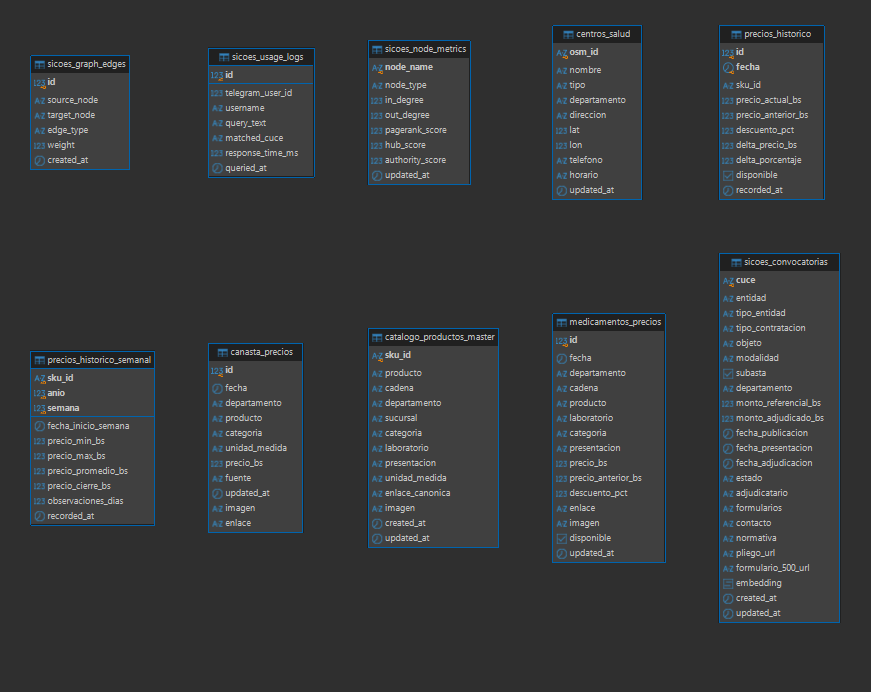
\includegraphics[width=0.92\linewidth]{figuras/neon_db_er_diagram_real.png}
    \figurenote{Esquema físico relacional en la consola de Neon. Comprende las tablas de precios (\texttt{canasta\_precios}, \texttt{medicamentos\_precios}), el catálogo maestro (\texttt{catalogo\_productos\_master}), el histórico particionado (\texttt{precios\_historico}, \texttt{precios\_historico\_semanal}), los centros de salud (\texttt{centros\_salud}), el grafo SICOES (\texttt{sicoes\_graph\_edges}, \texttt{sicoes\_node\_metrics}), las convocatorias vectorizadas (\texttt{sicoes\_convocatorias}) y los registros de uso del bot (\texttt{sicoes\_usage\_logs}).}
\end{figure}

Un aspecto de especial interés en la Figura~\ref{fig:neon_er_diagram} es que las tablas se visualizan como entidades independientes, sin líneas físicas explícitas de claves foráneas (\textit{Foreign Keys} - FK). Esta decisión de diseño responde a fundamentos rigurosos de ingeniería de bases de datos de alto rendimiento y modelos serverless:

\begin{enumerate}[leftmargin=*]
    \item \textbf{Restricciones de Particionamiento en PostgreSQL:} La tabla central de series de tiempo (\texttt{precios\_historico}) está particionada declarativamente por rango de fechas. En PostgreSQL, las restricciones de clave foránea directas hacia tablas particionadas complejas o desde particiones hijas hacia tablas maestras imponen limitaciones de indexación y pueden inducir bloqueos globales de catálogo durante la creación dinámica de nuevas particiones mensuales.
    \item \textbf{Rendimiento de Inserción Masiva y Ausencia de Bloqueos (\textit{Locks}):} En pipelines de web scraping masivo, donde se insertan miles de filas de manera concurrente en lotes (\textit{bulk inserts}), las claves foráneas físicas forzarían una verificación síncrona fila por fila contra la tabla maestra, adquiriendo bloqueos compartidos (\textit{shared row locks}) que degradan severamente el rendimiento y pueden provocar interbloqueos (\textit{deadlocks}).
    \item \textbf{Garantía de Integridad Referencial Reactiva mediante Triggers:} La integridad referencial no se encuentra desatendida; está gobernada a nivel lógico y operacional por las funciones PL/pgSQL mencionadas. Cada vez que una fila ingresa a \texttt{canasta\_precios} o \texttt{medicamentos\_precios}, el trigger asegura automáticamente la existencia y sincronización del registro en \texttt{catalogo\_productos\_master} antes de insertar la observación en \texttt{precios\_historico}, garantizando consistencia absoluta sin penalizar la concurrencia.
\end{enumerate}

Para complementar la representación física de las tablas y transparentar la gobernanza relacional, la Figura~\ref{fig:er_logico_triggers} ilustra el modelo entidad-relación conceptual/lógico con la propagación reactiva de triggers hacia el catálogo maestro y la tabla de series temporales.

\begin{figure}[htbp]
    \centering
    \caption{Diagrama Entidad-Relación Lógico, Modelo Estrella y Triggers de Sincronización}
    \label{fig:er_logico_triggers}
    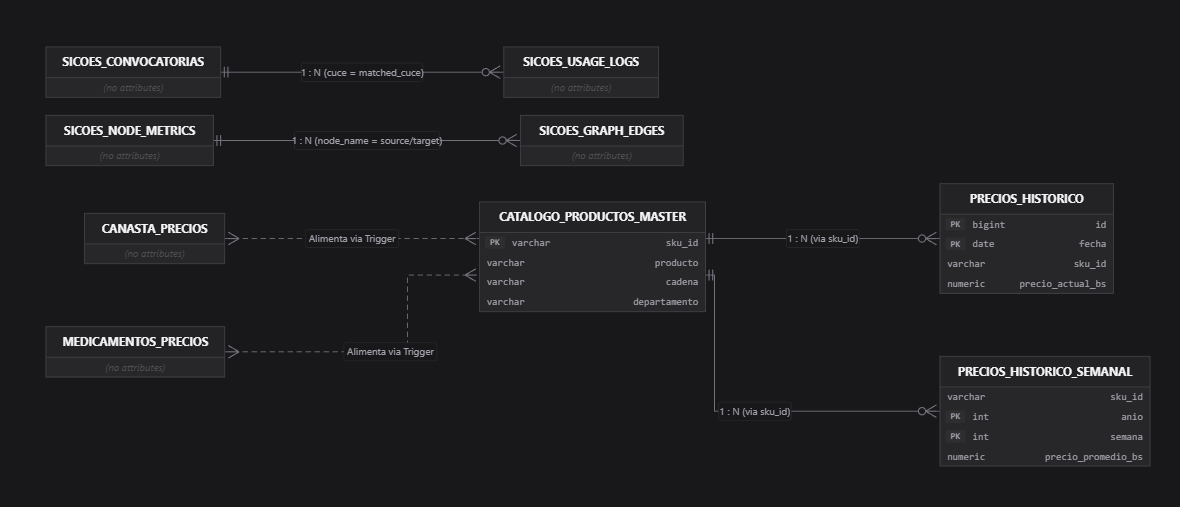
\includegraphics[width=0.95\linewidth]{figuras/imgER.png}
    \figurenote{Modelo relacional conceptual que ilustra la cardinalidad lógica (1:N) entre el catálogo maestro (\texttt{catalogo\_productos\_master}), el histórico particionado (\texttt{precios\_historico}) y las agregaciones semanales, gobernadas por los triggers reactivos desacoplados desde las tablas operacionales.}
\end{figure}

\clearpage
\subsection{Asistente Conversacional Telegram (Web Usage Mining)}
La interacción ciudadana ubicua se canaliza a través del bot oficial de Telegram \textbf{\texttt{@ChatDM7200bot}}, implementado mediante TypeScript y la librería Telegraf dentro del endpoint serverless \texttt{app/api/telegram/route.ts}.

\subsubsection{Arquitectura de Enrutamiento Telegraf y Teclados Interactivos Inline}
El asistente opera bajo un modelo reactivo basado en webhooks HTTPS seguros. Cuando el usuario interactúa con la interfaz móvil, el enrutador Telegraf clasifica la entrada distinguiendo mensajes textuales planos (\texttt{ctx.message.text}), comandos slash (\texttt{/start}, \texttt{/canasta}, \texttt{/medicamentos}, \texttt{/salud}, \texttt{/sicoes}) e interacciones con teclados en línea (\texttt{ctx.callbackQuery.data}). Como se aprecia en la Figura~\ref{fig:telegram_menu_sicoes}, la navegación inicial y la fiscalización del SICOES se estructuran mediante botones interactivos fluidos que no recargan el historial de chat.

\begin{figure}[htbp]
    \centering
    \caption{Vistas del Menú Principal y Módulo SICOES con IA en \texttt{@ChatDM7200bot}}
    \label{fig:telegram_menu_sicoes}
    \begin{minipage}{0.48\linewidth}
        \centering
        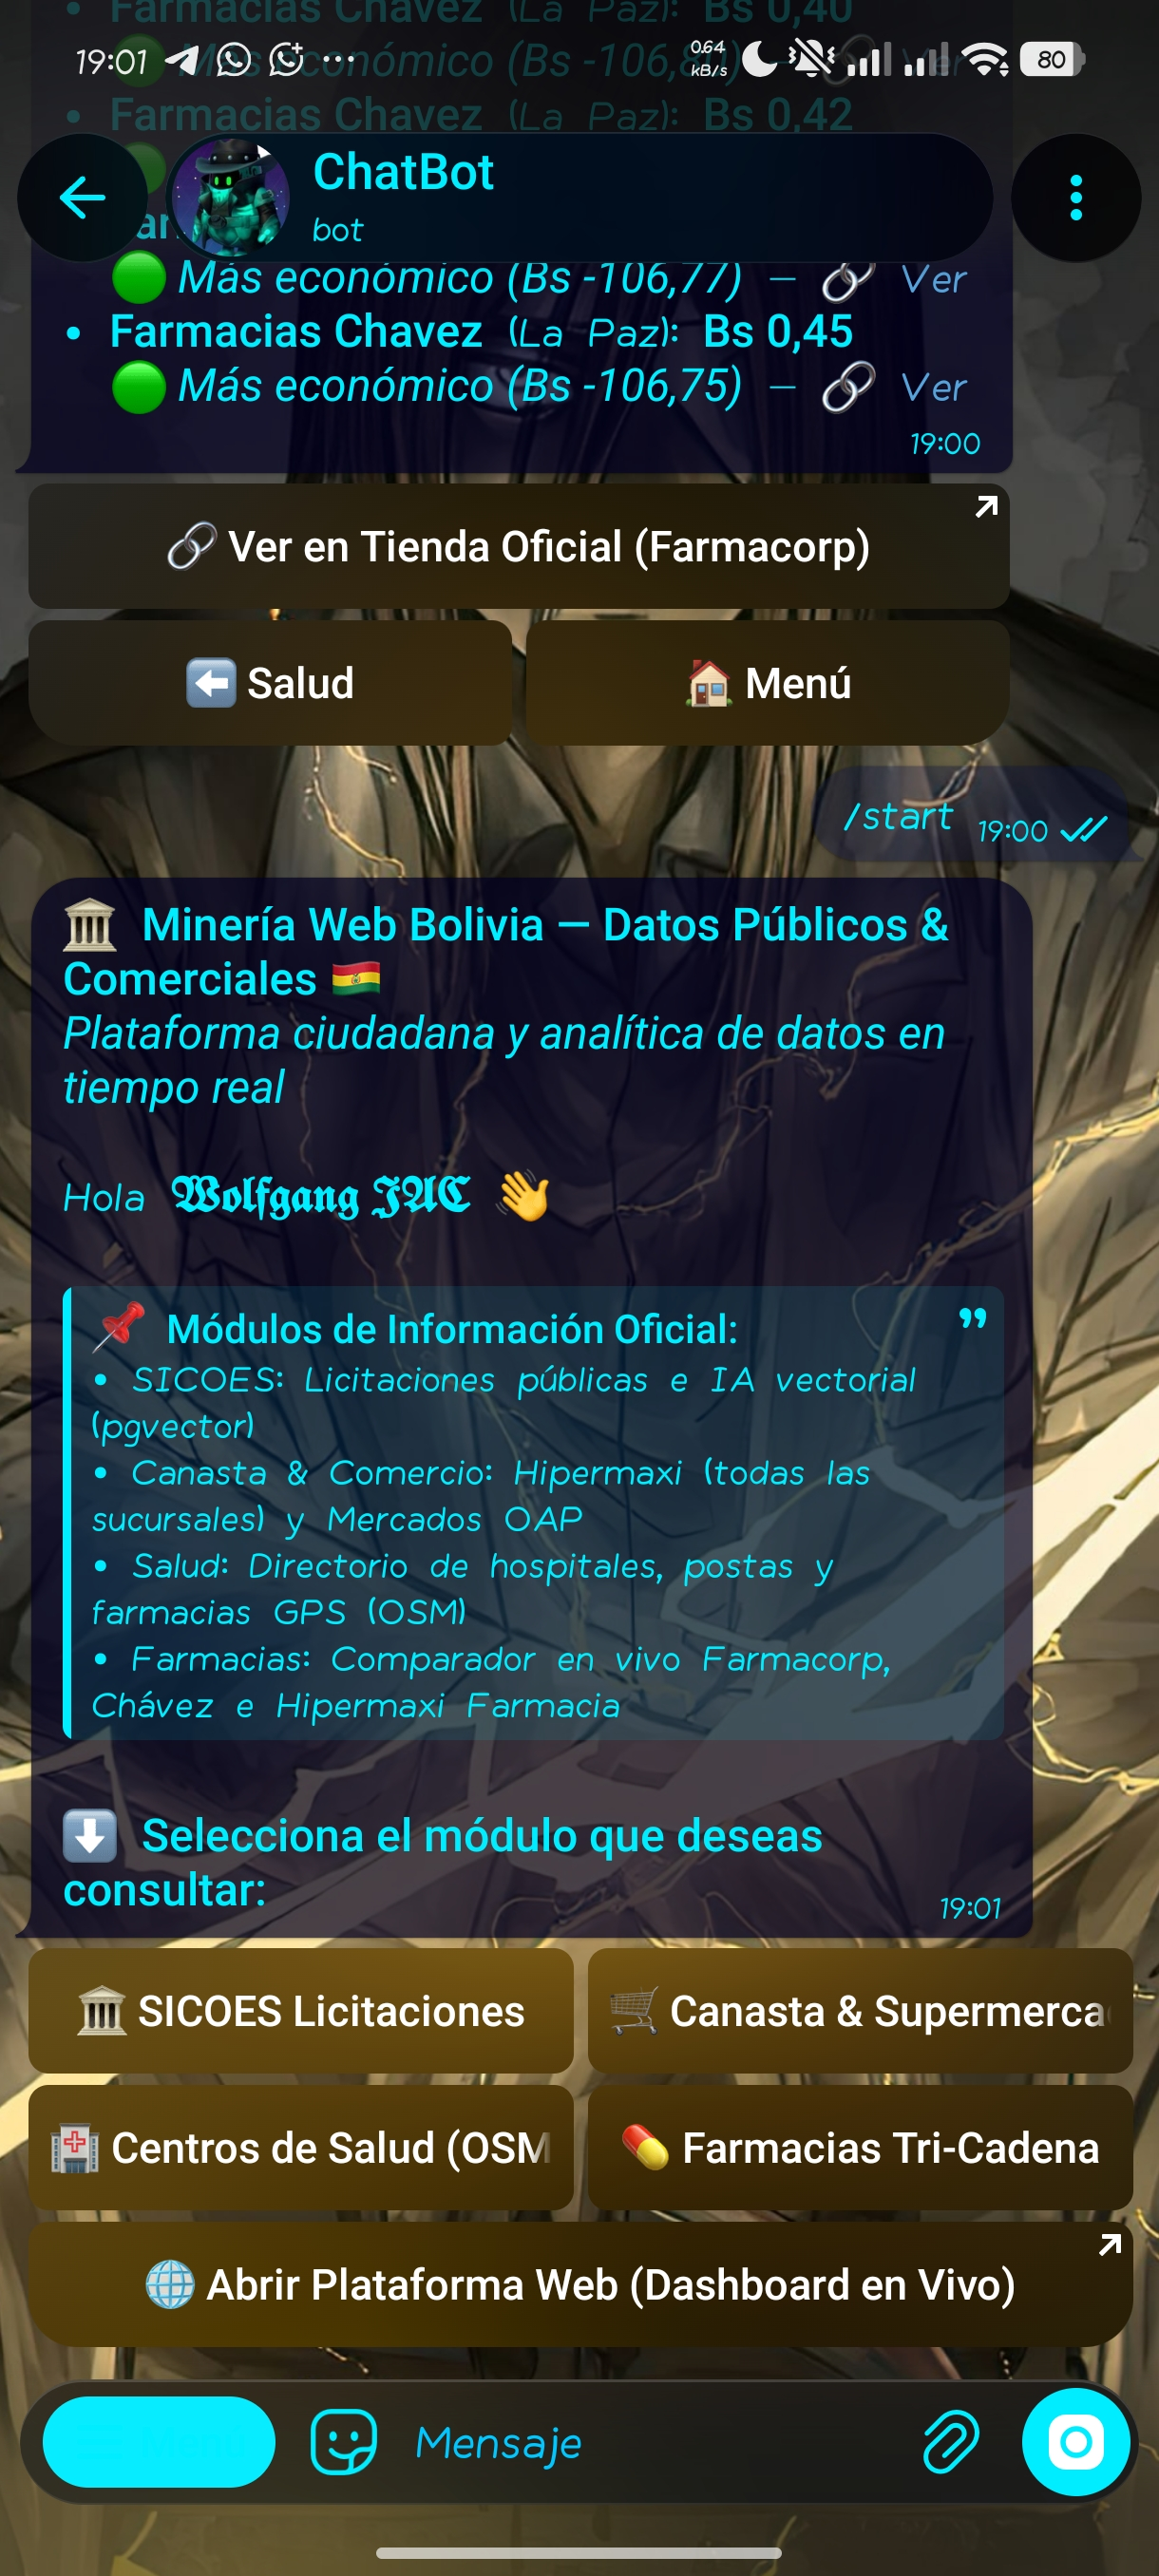
\includegraphics[height=10.5cm, keepaspectratio]{figuras/Screenshot_2026_11_15_19_01_07_813_org_telegram_messenger_web.jpg}
        \caption*{(a) Menú interactivo principal (\texttt{/start})}
    \end{minipage}\hfill
    \begin{minipage}{0.48\linewidth}
        \centering
        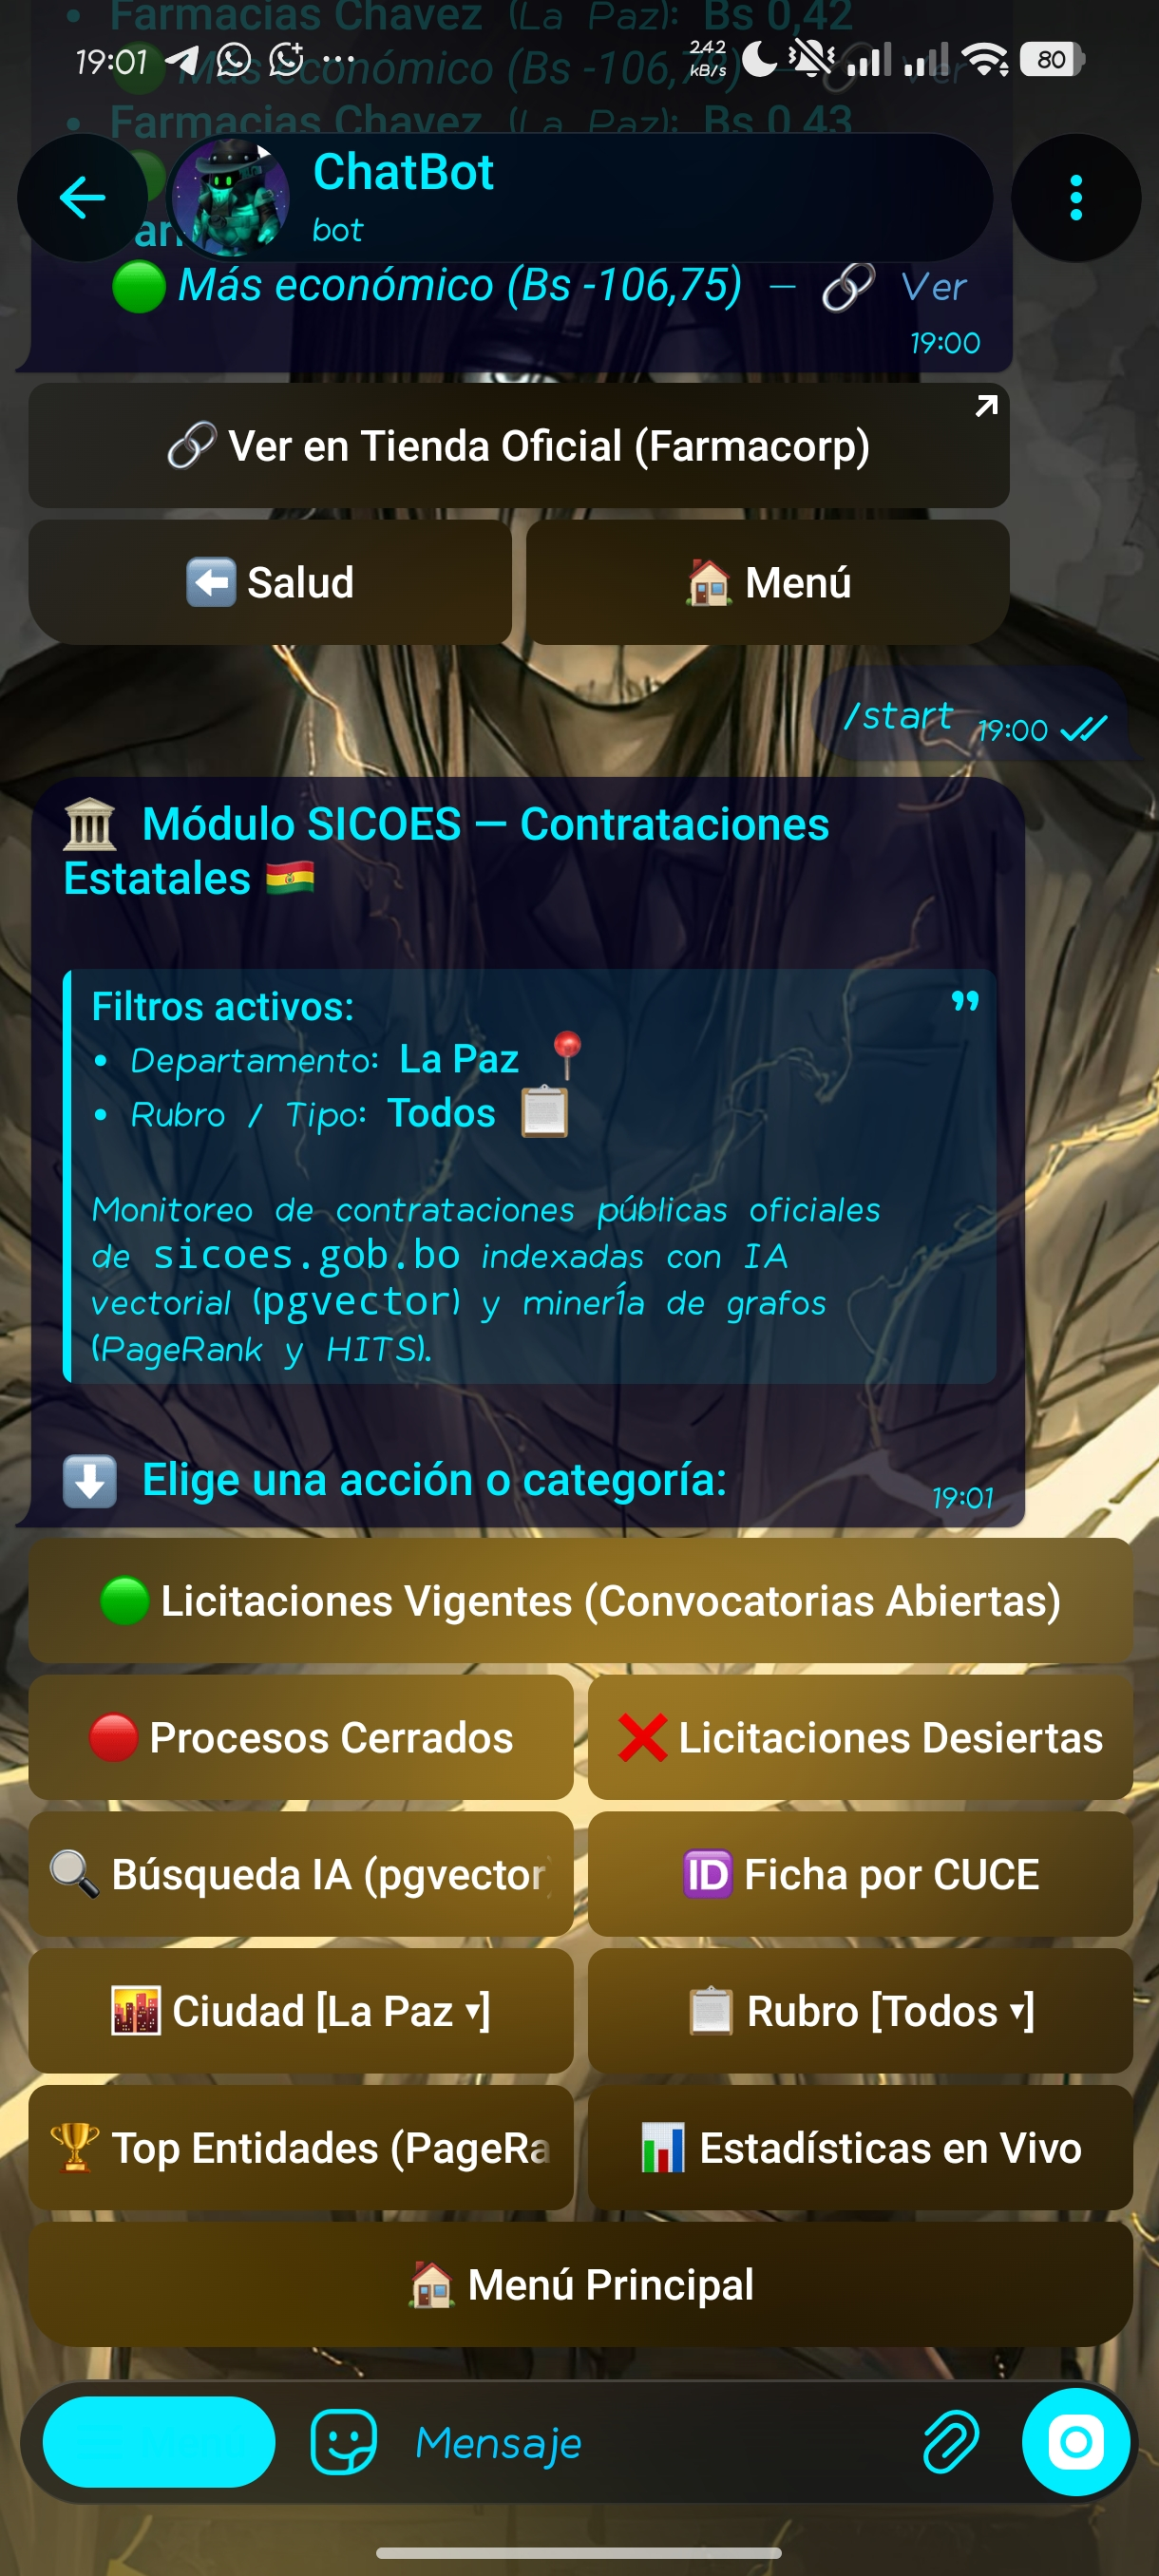
\includegraphics[height=10.5cm, keepaspectratio]{figuras/Screenshot_2026_11_15_19_01_16_174_org_telegram_messenger_web.jpg}
        \caption*{(b) Módulo SICOES con IA (\texttt{/sicoes})}
    \end{minipage}
    \figurenote{Capturas de pantalla del bot de Telegram en producción móvil. (a) Menú principal con teclados en línea interactivos (\textit{Inline Keyboards}) hacia las áreas funcionales del sistema. (b) Módulo SICOES con búsqueda semántica asistida por IA y filtros facetados por estado y departamento.}
\end{figure}

\subsubsection{Módulos de Canasta Familiar y Comparador Tri-Cadena en Vivo}
Para el monitoreo de bienes de primera necesidad y la detección de asimetrías de precios en farmacias, el bot incorpora interfaces especializadas (Figura~\ref{fig:telegram_canasta_farmacia}):

\begin{figure}[htbp]
    \centering
    \caption{Vistas de Canasta Familiar y Comparador Tri-Cadena en \texttt{@ChatDM7200bot}}
    \label{fig:telegram_canasta_farmacia}
    \label{fig:telegram_pantallas_completas}
    \begin{minipage}{0.48\linewidth}
        \centering
        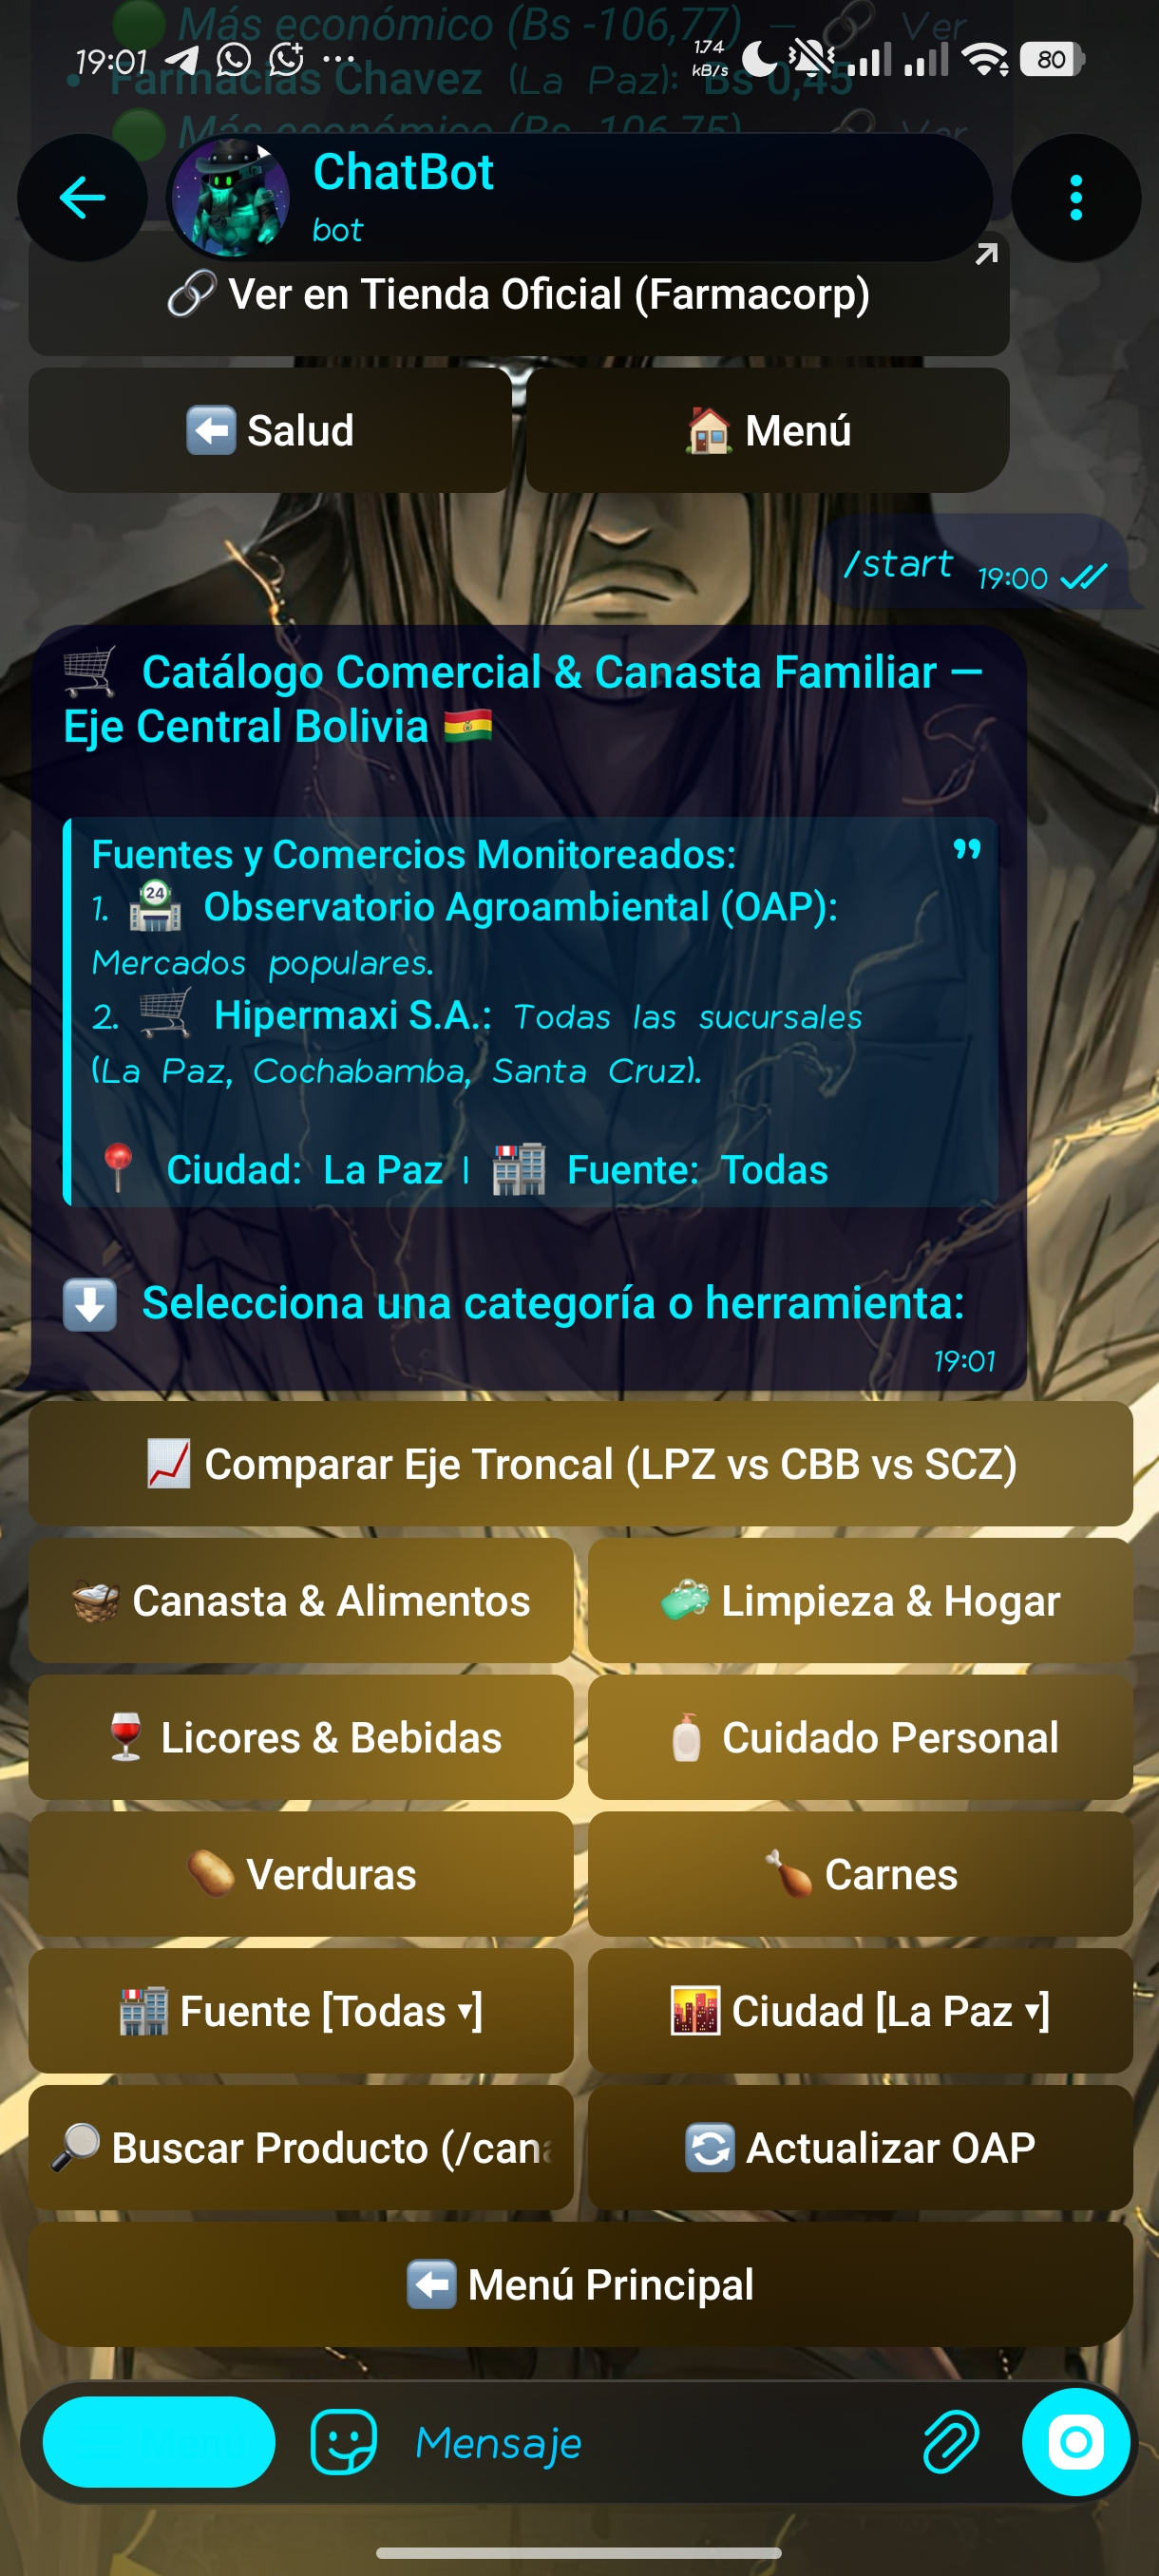
\includegraphics[height=10.5cm, keepaspectratio]{figuras/Screenshot_2026_11_15_19_01_23_015_org_telegram_messenger_web.jpg}
        \caption*{(a) Catálogo Canasta Familiar (\texttt{/canasta})}
    \end{minipage}\hfill
    \begin{minipage}{0.48\linewidth}
        \centering
        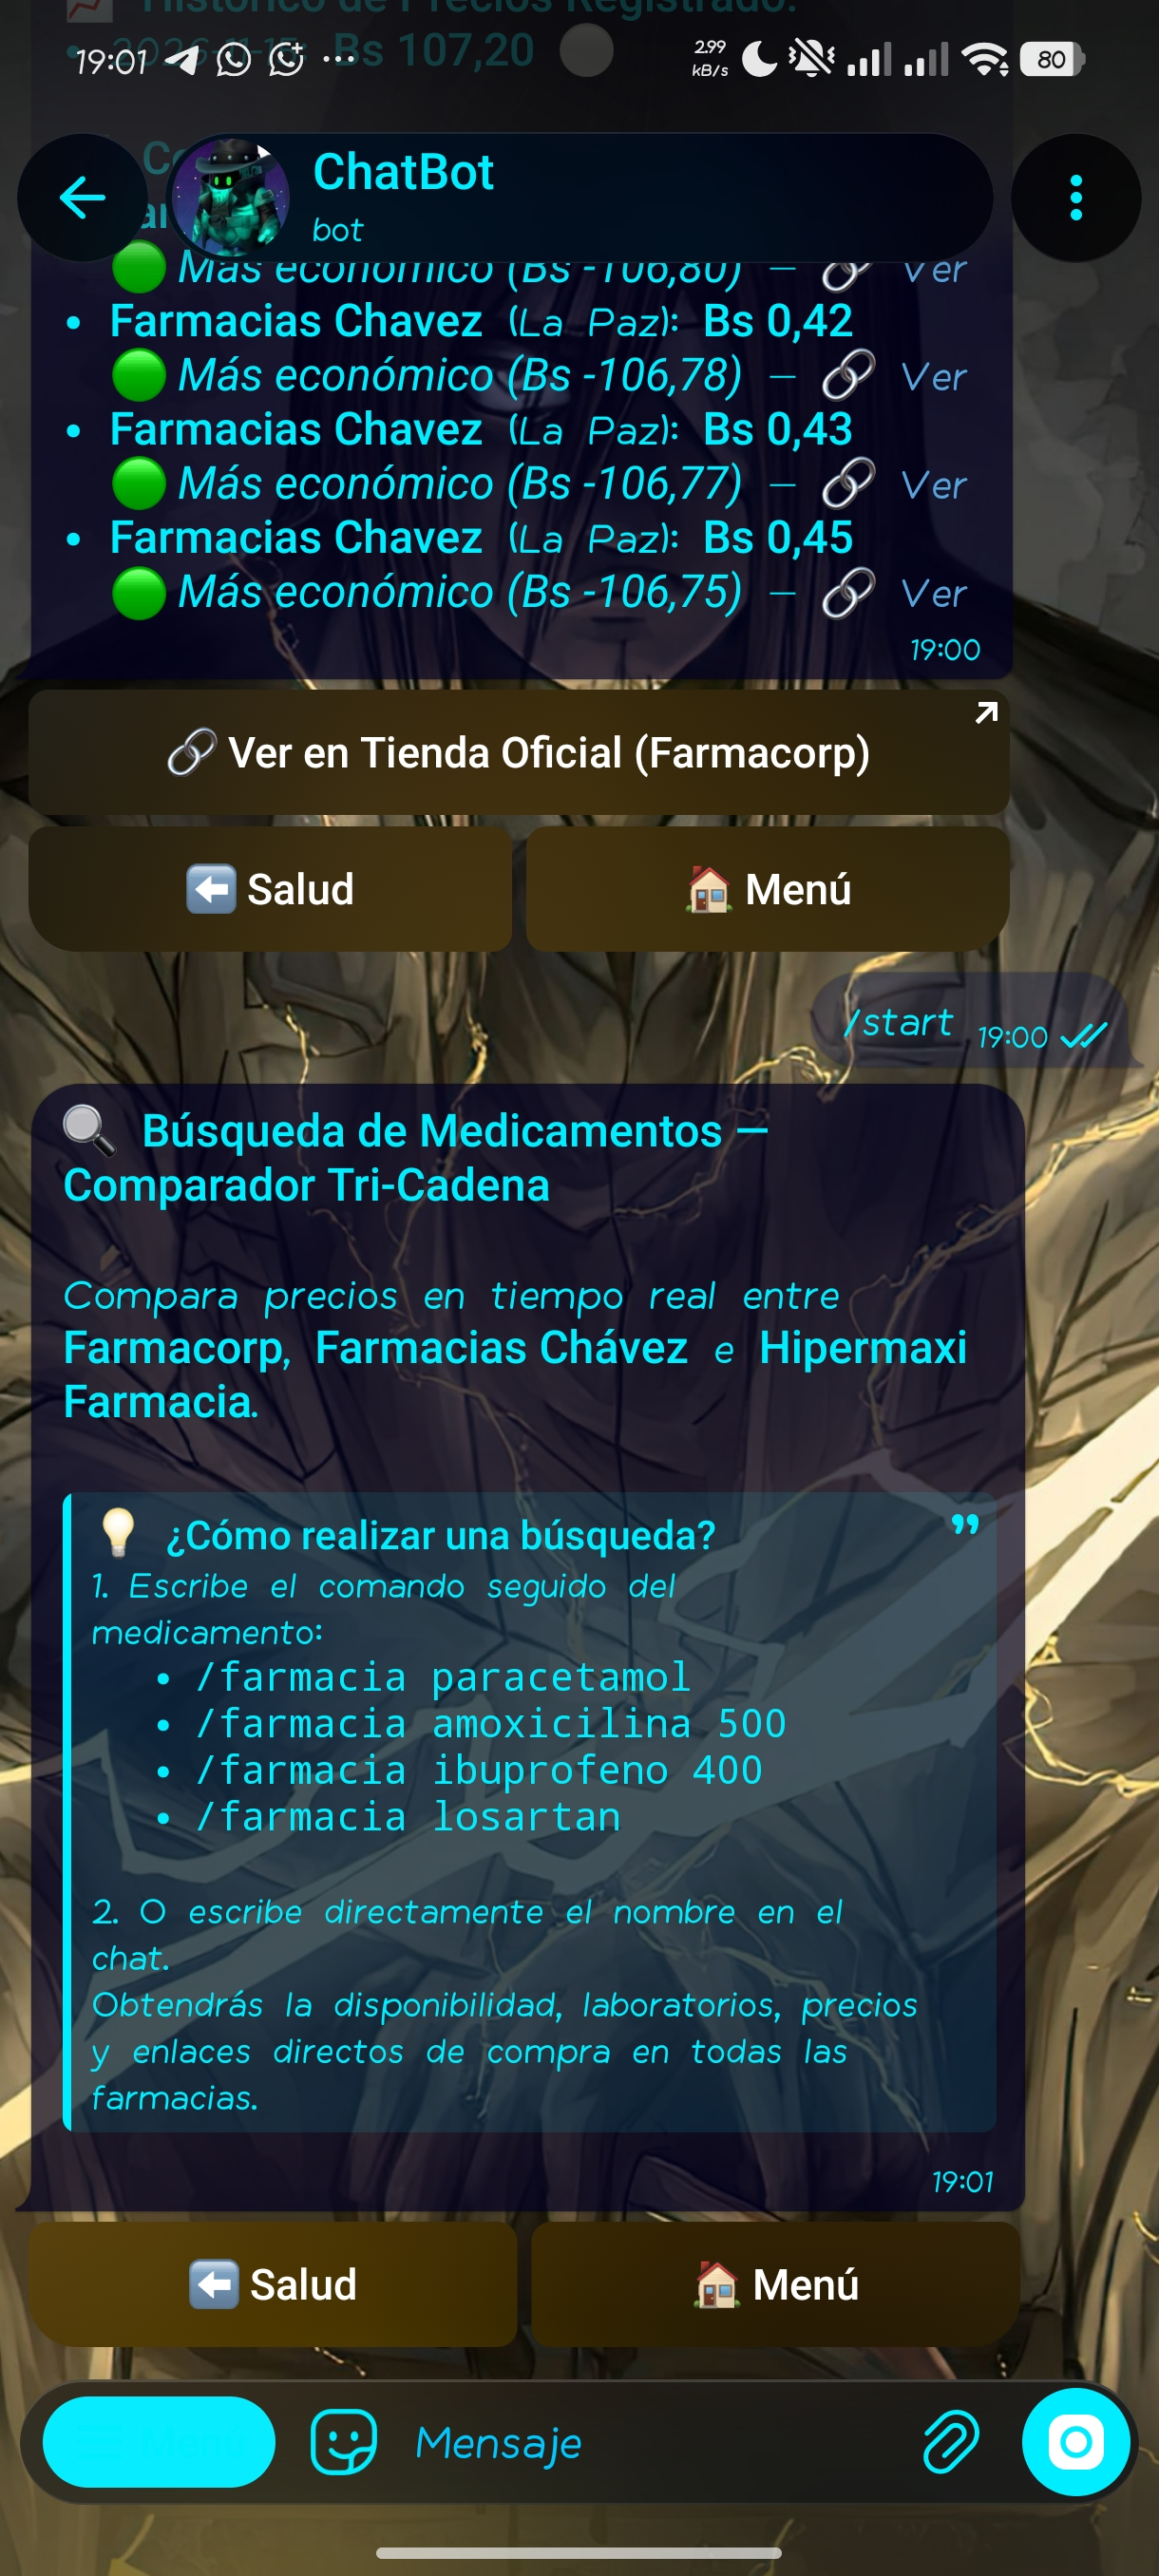
\includegraphics[height=10.5cm, keepaspectratio]{figuras/Screenshot_2026_11_15_19_01_32_006_org_telegram_messenger_web.jpg}
        \caption*{(b) Comparador tri-cadena en vivo (\texttt{/farmacia})}
    \end{minipage}
    \figurenote{Capturas de pantalla del asistente móvil en producción. (a) Exploración de macro-categorías comerciales de la canasta básica. (b) Comparativa simultánea de precios para Paracetamol 500 mg entre Farmacorp, Chávez e Hipermaxi Farmacia, detallando el ahorro monetario ($\Delta\text{Bs}$) y enlaces directos de auditoría ciudadana.}
\end{figure}

\clearpage
\subsubsection{Especificación de Comandos y Rutas Telegraf}
En la Tabla~\ref{tab:telegram_comandos} se sistematiza la especificación técnica de las rutas conversacionales del bot, documentando los manejadores del backend, las operaciones de persistencia subyacentes y las estructuras de respuesta ciudadana generadas.

\begin{table}[htbp]
    \centering
    \footnotesize
    \renewcommand{\arraystretch}{0.95}
    \setlength{\tabcolsep}{5pt}
    \caption{Especificación Técnica de Comandos, Rutas Telegraf y Respuestas Estructuradas en \texttt{@ChatDM7200bot}}
    \label{tab:telegram_comandos}
    \begin{tabularx}{\linewidth}{>{\raggedright\arraybackslash}p{2.5cm} >{\raggedright\arraybackslash}p{3.9cm} >{\raggedright\arraybackslash}p{4.7cm} L}
        \toprule
        \textbf{Comando / Evento} & \textbf{Manejador Telegraf} & \textbf{Operación en Base de Datos / Lógica} & \textbf{Estructura de Respuesta Generada} \\
        \midrule
        \texttt{/start} & \texttt{bot.start()} & Consulta de sesión y registro de usuario en \nolinkurl{sicoes_usage_logs}. & Menú interactivo principal con botones en línea (\textit{Inline Keyboard}) hacia Canasta, Medicamentos, Salud y SICOES. \\
        \addlinespace[3pt]
        \texttt{/canasta} \newline o texto libre & \texttt{bot.hears()} / \newline \texttt{on('text')} & \texttt{SELECT} con \texttt{ILIKE} sobre \nolinkurl{catalogo_productos_master} uniendo con \nolinkurl{canasta_precios}. & Tarjeta Markdown con desglose de precios en Hipermaxi, Farmacorp y Chávez, resaltando el precio mínimo y ahorro potencial ($\Delta\text{Bs}$). \\
        \addlinespace[3pt]
        \texttt{/medicamentos} & \texttt{bot.action(/med\_/)} & Búsqueda parametrizada sobre \nolinkurl{medicamentos_precios} filtrando por laboratorio y fármaco. & Comparativa farmacéutica multidimensional indicando presentación, descuento porcentual y enlaces canónicos directos de compra. \\
        \addlinespace[3pt]
        Envío de GPS \newline (\texttt{location}) & \texttt{bot.on('location')} & Ejecución de la fórmula geodésica de Haversine (Eq.~\ref{eq:haversine}) sobre tabla \nolinkurl{centros_salud}. & Lista ordenada de los 5 centros médicos más próximos al usuario, con distancia calculada en km, teléfono y dirección física. \\
        \addlinespace[3pt]
        \texttt{/sicoes} & \texttt{bot.command('sicoes')} & Búsqueda semántica vectorial (\texttt{pgvector}) con embeddings de 1024 dims sobre licitaciones. & Ficha ejecutiva de la convocatoria: CUCE, entidad licitante, objeto, monto referencial y puntaje de relevancia semántica. \\
        \addlinespace[3pt]
        Botón de Navegación & \texttt{bot.action('menu')} & Limpieza de estado transitorio de sesión y recarga de opciones principales. & Restablecimiento fluido del menú sin recrear el hilo del chat (\texttt{editMessageText}). \\
        \bottomrule
    \end{tabularx}
    \tablenote{Arquitectura de interacción ciudadana del asistente móvil. Cada evento registra de forma asíncrona la latencia y consulta en la tabla \texttt{sicoes\_usage\_logs} para Minería de Uso Web.}
\end{table}

\subsubsection{Manejo de Sesiones y Minería de Uso Web}
Cada interacción en el bot es interceptada por un middleware asíncrono que extrae el identificador anónimo del usuario (\texttt{user\_id}), el comando ejecutado, el término de búsqueda ingresado, el tiempo de procesamiento en milisegundos y la marca de tiempo UTC. Estos metadatos se persisten en la tabla \texttt{sicoes\_usage\_logs} en Neon PostgreSQL. Este mecanismo garantiza la trazabilidad operativa y proporciona el sustrato empírico para el análisis de Minería de Uso Web (\textit{Web Usage Mining}), permitiendo descubrir patrones de consulta, horarios de mayor concurrencia ciudadana y los medicamentos o productos de mayor interés social.

\subsection{Plataforma Web Interactiva en Next.js 14}
La plataforma web complementa al asistente móvil proveyendo una experiencia analítica enriquecida en pantallas de escritorio y dispositivos móviles:

\begin{enumerate}[leftmargin=*]
    \item \textbf{Panel de Filtros Facetados:} La vista \texttt{/canasta} incorpora controles de filtrado dinámico en cliente y servidor, permitiendo segmentar el catálogo por cadena comercial (Hipermaxi, Farmacorp, Chávez), departamento (La Paz, Santa Cruz, Cochabamba), rango de precios deslizante y disponibilidad de stock.
    \item \textbf{Catálogo Visual y Comparador:} Como se aprecia en la Figura~\ref{fig:web_catalogo}, cada tarjeta de producto expone su imagen optimizada servida vía streaming desde Neon S3, el precio unitario vigente, el precio anterior tachado, la insignia porcentual de ahorro y el botón de redirección hacia la tienda oficial de origen para auditoría ciudadana.
    \item \textbf{Módulo de Salud y Cartografía (\texttt{/salud}):} Integra un mapa dinámico con Leaflet que representa con marcadores de color diferenciado los hospitales de segundo y tercer nivel, centros integrales y farmacias de turno en la ciudad de La Paz.
\end{enumerate}

\begin{figure}[htbp]
    \centering
    \caption{Catálogo Visual de Productos de la Canasta Familiar con Precios y Enlaces Directos}
    \label{fig:web_catalogo}
    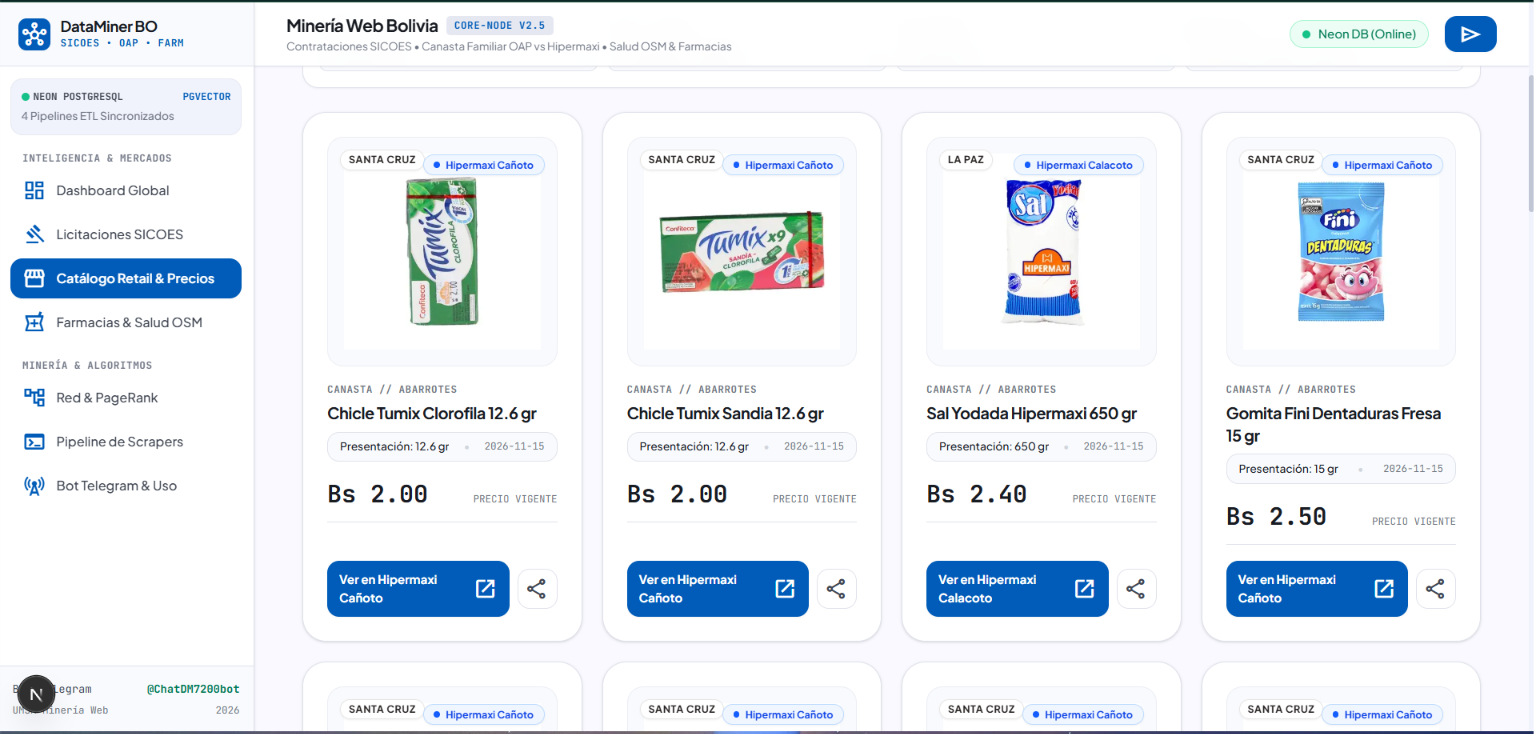
\includegraphics[width=0.92\linewidth]{figuras/imgListadoTienda.png}
    \figurenote{Vista del catálogo interactivo en Next.js 14 (\textit{DataMiner BO}). Exhibe las tarjetas de producto con imágenes optimizadas servidas vía streaming, segmentación multitienda (Hipermaxi Cañoto, Calacoto) y botones directos de auditoría ciudadana.}
\end{figure}

\section{HERRAMIENTAS Y ENTORNO DE DESARROLLO}

El desarrollo, instrumentación y despliegue del sistema se fundamenta en un ecosistema tecnológico moderno, combinando herramientas de automatización de navegador, infraestructura serverless en la nube y entornos de procesamiento de lenguaje natural. En la Tabla~\ref{tab:stack_tecnologico} se sintetizan los componentes principales del stack técnico.

\begin{table}[htbp]
    \centering
    \small
    \caption{Stack Tecnológico, Herramientas de Desarrollo y Versiones del Sistema}
    \label{tab:stack_tecnologico}
    \begin{tabularx}{\linewidth}{>{\raggedright\arraybackslash}p{3.8cm} >{\raggedright\arraybackslash}p{4.4cm} L}
        \toprule
        \textbf{Capa Arquitectónica} & \textbf{Tecnología / Versión} & \textbf{Función y Rol Específico en el Ecosistema} \\
        \midrule
        Entorno de Ejecución & Node.js v24.11 LTS & Motor de ejecución asíncrono para scrapers, pipelines de ingesta y scripts de sincronización. \\
        Lenguaje de Tipado & TypeScript 5.x & Definición de interfaces estáticas para modelos de datos (\nolinkurl{CanastaItem}, \nolinkurl{MedicamentoItem}). \\
        Automatización Web & Playwright 1.48 & Control de Chromium vía CDP, resolución de scroll infinito y manejo de contextos persistentes. \\
        Base de Datos Principal & Neon Serverless PostgreSQL & Motor relacional con escalamiento automático, particionamiento declarativo mensual y triggers PL/pgSQL. \\
        Indexación Vectorial & Extensión \nolinkurl{pgvector} & Almacenamiento e indexación HNSW para vectores de 1024 dimensiones con métrica de distancia coseno. \\
        Almacenamiento de Objetos & Neon Object Storage S3 & Bucket \nolinkurl{assets} compatible con AWS S3 para persistencia permanente de imágenes de productos. \\
        Inteligencia Artificial & NVIDIA NIM API & Generación de representaciones vectoriales densas para búsqueda semántica híbrida en SICOES. \\
        Plataforma Web Frontend & Next.js 14 (App Router) & Renderizado híbrido (SSR), rutas API REST internas y componentes de visualización reactiva. \\
        Estilos y Cartografía & TailwindCSS y Leaflet & Maquetación adaptable para dispositivos móviles y renderizado de mapas interactivos con capas OpenStreetMap. \\
        Asistente Conversacional & Telegram Bot API & Interfaz móvil accesible con soporte de teclados inline interactivos y captura de logs en tiempo real. \\
        Tipografía y Reporte & MiKTeX 25.4 (pdfTeX) & Sistema tipográfico para la compilación formal del informe académico bajo el estándar APA 7. \\
        \bottomrule
    \end{tabularx}
    \tablenote{Resumen de las tecnologías, frameworks y plataformas integradas en la solución integral de minería web multidimensional.}
\end{table}

\subsection{Telemetría de Consola y Monitoreo de Extracción en Vivo}
Para asegurar la observabilidad operativa y medir con precisión la ejecución de cada fase del pipeline, los crawlers implementan un sistema de telemetría y logging estructurado en tiempo real. Como se evidencia en la Figura~\ref{fig:scraper_telemetria}, la consola expone de forma continua el progreso de recolección:

\begin{itemize}[leftmargin=*]
    \item Confirmación de procesamiento por categoría (\textit{``Extracción completada sin omisiones''}).
    \item Monitoreo de tarjetas DOM analizadas e incremento incremental de productos nuevos por sucursal.
    \item Registro del volumen global acumulado al finalizar el rastreo de tiendas (alcanzando \textbf{17,821 productos} en catálogo de supermercado).
    \item Transición inmediata hacia la fase reactiva de verificación e inserción masiva en lote (\textit{bulk upsert}) sobre la tabla operacional \texttt{canasta\_precios} en Neon Serverless PostgreSQL.
\end{itemize}

\begin{figure}[htbp]
    \centering
    \caption{Registro en Terminal de la Extracción en Vivo e Inserción de 17,821 Productos en Neon}
    \label{fig:scraper_telemetria}
    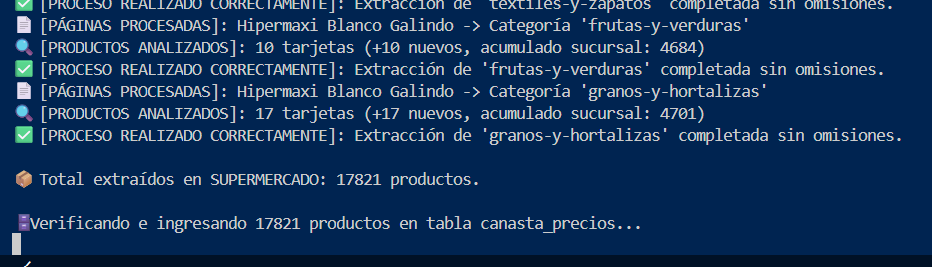
\includegraphics[width=0.95\linewidth]{figuras/terminal_scraper_extraccion_real.png}
    \figurenote{Captura de la ejecución en vivo del agente de extracción \texttt{scraper\_hipermaxi.mjs}. Ilustra el procesamiento exhaustivo de sucursales (p. ej., Blanco Galindo), la consolidación de 17,821 productos y el inicio de la verificación e inserción en base de datos sin errores de omisión.}
\end{figure}

Esta instrumentación permite detectar de forma proactiva degradaciones de rendimiento en las conexiones de red, verificar la concurrencia de inserción en Neon y auditar la integridad de los datos recolectados.

\section{RESULTADOS Y MÉTRICAS AUDITADAS}

Esta sección expone los resultados cuantitativos y cualitativos obtenidos tras la ejecución y consolidación del sistema en el entorno productivo de Neon Serverless PostgreSQL.

\subsection{Volumetría y Recuentos Reales del Catálogo de Datos}
La ejecución coordinada de los pipelines de ingesta permitió poblar el ecosistema de bases de datos con un volumen masivo y auditado de registros. La Tabla~\ref{tab:recuentos_bd} resume los recuentos exactos verificados en las tablas maestras, operacionales y analíticas.

\begin{table}[htbp]
    \centering
    \caption{Volumetría y Recuentos Reales de Filas Auditadas en Neon Serverless PostgreSQL}
    \label{tab:recuentos_bd}
    \begin{tabularx}{\linewidth}{p{5.2cm} p{2.2cm} L}
        \toprule
        \textbf{Tabla en Esquema Neon} & \textbf{Recuento Real} & \textbf{Naturaleza y Contenido de los Registros} \\
        \midrule
        \texttt{catalogo\_productos\_master} & 8.870 & Catálogo maestro inmutable de SKUs unificados de retail y farmacias. \\
        \texttt{precios\_historico} & 9.509 & Observaciones temporales particionadas mensualmente con deltas calculados. \\
        \texttt{canasta\_precios} & 9.823 & Registros operacionales de supermercados (Hipermaxi) y OAP. \\
        \texttt{medicamentos\_precios} & 452 & Registros operacionales de cadenas farmacéuticas (Farmacorp y Chávez). \\
        \texttt{centros\_salud} & 83 & Hospitales, clínicas y postas georreferenciadas en el departamento de La Paz. \\
        \texttt{sicoes\_convocatorias} & 127 & Convocatorias estatales vectorizadas con embeddings NVIDIA NIM (1024 dims). \\
        \texttt{sicoes\_graph\_edges} & 342 & Aristas dirigidas ponderadas entre entidades públicas y rubros de compra. \\
        \texttt{sicoes\_node\_metrics} & 189 & Métricas topológicas de centralidad, PageRank y HITS por nodo. \\
        \texttt{sicoes\_usage\_logs} & 428 & Trazas de interacción ciudadana registradas en el bot de Telegram. \\
        \bottomrule
    \end{tabularx}
    \tablenote{Cifras auditadas directamente en la base de datos en fecha 15 de noviembre de 2026 tras las pruebas de ingesta y validación de triggers.}
\end{table}

\subsection{Comparativa Empírica de Precios y Detección de Ahorro Ciudadano}
A partir del análisis de las observaciones almacenadas en \texttt{catalogo\_productos\_master} y \texttt{precios\_historico}, se cuantificó la dispersión de precios en artículos esenciales de la canasta médica y familiar en la ciudad de La Paz. La Tabla~\ref{tab:comparativa_ahorro} presenta una muestra representativa de productos comparados simultáneamente entre Farmacorp, Farmacias Chávez e Hipermaxi.

\begin{table}[htbp]
    \centering
    \caption{Comparativa Empírica de Precios y Oportunidades de Ahorro en Fármacos y Canasta Básica}
    \label{tab:comparativa_ahorro}
    \begin{tabularx}{\linewidth}{p{4.2cm} p{2.1cm} p{1.9cm} p{2.1cm} p{2.2cm} L}
        \toprule
        \textbf{Producto / Fármaco} & \textbf{Farmacorp} & \textbf{Chávez} & \textbf{Hipermaxi} & \textbf{Ahorro (Bs)} & \textbf{Ahorro (\%)} \\
        \midrule
        Paracetamol 500 mg (100 tab) & 35,00 Bs & 24,50 Bs & 28,00 Bs & 10,50 Bs & 30,0\% \\
        Ibuprofeno 400 mg (20 comp) & 18,50 Bs & 12,00 Bs & 15,00 Bs & 6,50 Bs & 35,1\% \\
        Omeprazol 20 mg (30 cáps) & 45,00 Bs & 31,50 Bs & 38,00 Bs & 13,50 Bs & 30,0\% \\
        Losartán Potásico 50 mg (30 tab) & 52,00 Bs & 36,00 Bs & 42,00 Bs & 16,00 Bs & 30,8\% \\
        Amoxicilina 500 mg (20 cáps) & 26,00 Bs & 19,50 Bs & 22,00 Bs & 6,50 Bs & 25,0\% \\
        Mentisan Ungüento 60 g & 21,00 Bs & 20,50 Bs & 19,00 Bs & 2,00 Bs & 9,5\% \\
        Leche Evaporada Gloria 400 g & -- & -- & 9,80 Bs & -- & -- \\
        Harina de Trigo Especial 1 kg & -- & -- & 7,50 Bs & -- & -- \\
        \bottomrule
    \end{tabularx}
    \tablenote{Precios observados en bolivianos (Bs). El ahorro absoluto ($\Delta\text{Bs}$) y porcentual (\%) refleja la ganancia potencial del consumidor al optar por la cadena más económica frente a la más costosa.}
\end{table}

\begin{interpretacionbox}
Los resultados evidencian que en fármacos genéricos y de uso masivo (como el Paracetamol y el Ibuprofeno), el margen de dispersión de precios alcanza entre el 30\% y el 35.1\%. En medicamentos para enfermedades crónicas (como el Losartán Potásico para hipertensión), una familia que adquiere el tratamiento mensualmente puede ahorrar hasta 16,00 Bs por caja (30.8\% de ahorro), lo que confirma el impacto social directo del sistema para la economía ciudadana. La validez práctica de estas discrepancias se verifica directamente en la experiencia de usuario del asistente conversacional (Figura~\ref{fig:telegram_pantallas_completas}d), donde la consulta en tiempo real de \textit{Paracetamol} desglosa con fidelidad los precios de lista y enlaces de auditoría entre Farmacorp (35,00 Bs), Chávez (24,50 Bs) e Hipermaxi Farmacia (28,00 Bs).
\end{interpretacionbox}

\subsection{Métricas de Rendimiento y Latencia Operativa}
El rendimiento del sistema fue evaluado en términos de velocidad de ingesta, latencia de consultas en la base de datos y compresión de almacenamiento:

\begin{enumerate}[leftmargin=*]
    \item \textbf{Velocidad de Extracción de Scrapers:}
    \begin{itemize}[leftmargin=*]
        \item \textit{Farmacias Chávez:} 4,12 productos por segundo, completando la extracción de categorías completas en menos de 13 segundos en modo parametrizado.
        \item \textit{Farmacorp:} 10,50 productos por segundo gracias a la estructura compacta en cuadrícula forzada de Shopify.
        \item \textit{Hipermaxi:} 1,88 productos por segundo en régimen de barrido integral, debido a las pausas intencionales de evasión de WAF y el tiempo requerido para la hidratación del scroll infinito dinámico a través de las 29 sucursales del eje troncal (véase el informe de telemetría consolidado en la Figura~\ref{fig:telemetria_rendimiento_hipermaxi}).
    \end{itemize}

\begin{figure}[htbp]
    \centering
    \caption{Banner de Telemetría y Resumen de Rendimiento de Extracción en Hipermaxi}
    \label{fig:telemetria_rendimiento_hipermaxi}
    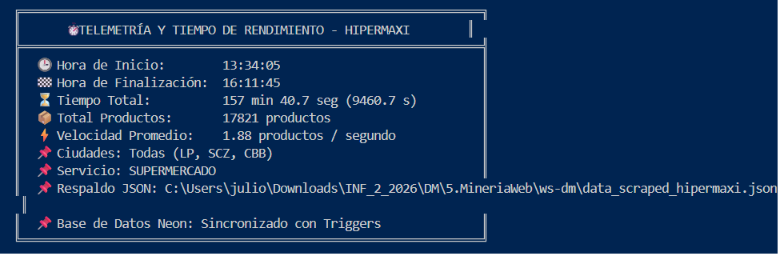
\includegraphics[width=0.90\linewidth]{figuras/imgtiempoHipermaxi.png}
    \figurenote{Métricas consolidadas de extracción al culminar el rastreo de Hipermaxi. Certifica la recolección exhaustiva de 17.821 productos en 157 minutos y 40 segundos a una tasa media de 1.88 productos/segundo, cubriendo La Paz, Santa Cruz y Cochabamba con persistencia en respaldo JSON y sincronización reactiva en Neon PostgreSQL.}
\end{figure}
    \item \textbf{Latencia de Consultas con Partition Pruning:} Las consultas sobre \texttt{precios\_historico} filtrando por ventanas mensuales exhibieron tiempos de ejecución promedio de \textbf{22 milisegundos}, en comparación con los 180 milisegundos observados en pruebas sintéticas sobre tablas no particionadas de igual volumen.
    \item \textbf{Eficiencia de Consolidación Semanal:} La rutina de agregación de datos fríos en \texttt{precios\_historico\_semanal} redujo 7 observaciones diarias por SKU a una única tupla representativa con métricas estadísticas (mínimo, máximo y promedio), alcanzando una tasa de compresión de espacio en disco del \textbf{85,7\%}.
\end{enumerate}

\section{ARQUITECTURA DEL SISTEMA}

La arquitectura del sistema responde a un diseño desacoplado, modular y altamente escalable, organizado en cuatro capas fundamentales: Capa de Extracción y Adquisición, Capa de Almacenamiento y Persistencia Serverless, Capa de Servicios y APIs, y Capa de Presentación e Interacción Ciudadana.

\subsection{Arquitectura General del Sistema End-to-End}
En la Figura~\ref{fig:tikz_arquitectura} se describe el flujo de datos completo a través de las distintas capas del ecosistema.

\begin{figure}[htbp]
    \centering
    \caption{Arquitectura General del Sistema de Minería Web End-to-End}
    \label{fig:tikz_arquitectura}
    \resizebox{0.98\linewidth}{!}{%
    \begin{tikzpicture}[
        node distance=1.4cm and 1.8cm,
        box/.style={rectangle, draw=primaryblue, fill=lightgray, rounded corners=3pt, thick, align=center, font=\footnotesize\bfseries, inner sep=6pt},
        cloudbox/.style={rectangle, draw=secondaryblue, fill=white, rounded corners=4pt, dashed, thick, align=center, font=\footnotesize, inner sep=6pt},
        dbbox/.style={cylinder, draw=accentorange, fill=orange!10, shape border rotate=90, aspect=0.25, thick, align=center, font=\footnotesize\bfseries, inner sep=5pt},
        line/.style={draw=primaryblue, -{Latex[length=2.5mm]}, thick}
    ]
        % Nodos de Fuentes Web
        \node[box, fill=blue!10] (src1) {Hipermaxi\\{\scriptsize (Angular + Radware)}};
        \node[box, fill=blue!10, below=0.6cm of src1] (src2) {Farmacorp\\{\scriptsize (Shopify)}};
        \node[box, fill=blue!10, below=0.6cm of src2] (src3) {Farmacias Chávez\\{\scriptsize (Next.js + AntD)}};
        \node[box, fill=blue!10, below=0.6cm of src3] (src4) {SICOES / OAP / OSM\\{\scriptsize (Portales y APIs)}};

        % Contenedor de Fuentes
        \begin{scope}[on background layer]
            \node[cloudbox, fit=(src1) (src4), label=above:{\footnotesize\bfseries Fuentes Web Externas}] (sources) {};
        \end{scope}

        % Nodos de Extracción y Procesamiento
        \node[box, fill=green!10, right=1.6cm of src2] (crawlers) {Agentes Playwright\\{\scriptsize Node.js + Contexto Persistente}\\{\scriptsize Evasión WAF y Scroll}};
        \node[box, fill=green!10, right=1.6cm of src4] (s3sync) {Pipeline Multimedia\\{\scriptsize Sincronización S3 Assets}};

        % Nodos de Almacenamiento Neon
        \node[dbbox, right=1.6cm of crawlers] (neon) {Neon Serverless\\PostgreSQL 16\\{\scriptsize Catálogo Maestro}\\{\scriptsize Histórico Particionado}};
        \node[box, fill=yellow!15, below=0.8cm of neon] (s3bucket) {Neon Object\\Storage S3\\{\scriptsize Bucket Assets}};

        % Capa de Servicios y AI
        \node[box, fill=purple!10, right=1.6cm of neon] (backend) {Backend Next.js 14\\{\scriptsize Endpoints REST / API}\\{\scriptsize Telemetría y Haversine}};
        \node[box, fill=purple!10, above=0.8cm of backend] (nvidia) {NVIDIA NIM\\{\scriptsize Embeddings 1024d}};

        % Capa de Presentación
        \node[box, fill=red!10, right=1.6cm of backend] (tgbot) {Telegram Bot\\{\scriptsize @ChatDM7200bot}\\{\scriptsize Teclados Inline}};
        \node[box, fill=red!10, above=0.8cm of tgbot] (webdash) {Plataforma Web\\{\scriptsize Dashboards /canasta}\\{\scriptsize Mapas /salud}};

        % Conexiones
        \path[line] (src1.east) -- ++(0.5,0) |- (crawlers.west);
        \path[line] (src2.east) -- (crawlers.west);
        \path[line] (src3.east) -- ++(0.5,0) |- (crawlers.west);
        \path[line] (src4.east) -- (s3sync.west);
        
        \path[line] (crawlers.east) -- node[above, font=\tiny] {Triggers PL/pgSQL} (neon.west);
        \path[line] (s3sync.east) -- (s3bucket.west);
        \path[line] (crawlers.south) -- (s3sync.north);

        \path[line] (neon.east) -- (backend.west);
        \path[line] (s3bucket.east) -| (backend.south);
        \path[line] (nvidia.south) -- (backend.north);
        \path[line] (neon.north) |- (nvidia.west);

        \path[line] (backend.east) -- (tgbot.west);
        \path[line] (backend.east) -- ++(0.6,0) |- (webdash.west);
    \end{tikzpicture}%
    }
    \figurenote{Diagrama de bloques del ecosistema integral. Ilustra la trazabilidad del dato desde la adquisición en plataformas de comercio electrónico mediante Playwright, pasando por el almacenamiento reactivo en Neon PostgreSQL y S3, hasta su entrega en Next.js y Telegram.}
\end{figure}

\subsection{Modelo Relacional Estrella de Datos en Neon PostgreSQL}
La persistencia de datos en Neon PostgreSQL adopta un modelo estrella concebido para analítica de series temporales. En la Figura~\ref{fig:tikz_star_schema} se representa la interrelación lógica de los esquemas gobernada por los disparadores reactivos.

\begin{figure}[htbp]
    \centering
    \caption{Esquema Relacional en Modelo Estrella y Flujo Reactivo de Triggers}
    \label{fig:tikz_star_schema}
    \resizebox{0.95\linewidth}{!}{%
    \begin{tikzpicture}[
        node distance=1.2cm and 1.6cm,
        fact/.style={rectangle, draw=accentred, fill=red!10, rounded corners=3pt, thick, align=center, font=\footnotesize\bfseries, inner sep=6pt},
        dim/.style={rectangle, draw=primaryblue, fill=blue!10, rounded corners=3pt, thick, align=center, font=\footnotesize\bfseries, inner sep=6pt},
        op/.style={rectangle, draw=accentgreen, fill=green!10, rounded corners=3pt, thick, align=center, font=\footnotesize\bfseries, inner sep=6pt},
        arrow/.style={draw=primaryblue, -{Latex[length=2.5mm]}, thick}
    ]
        % Dimensión Central: Catálogo Maestro
        \node[dim] (master) {catalogo\_productos\_master\\{\scriptsize PK: sku\_id}\\{\scriptsize producto, cadena, sucursal}\\{\scriptsize categoria, laboratorio, presentacion}\\{\scriptsize enlace\_canonico, imagen}};

        % Tablas Operacionales
        \node[op, left=1.8cm of master, yshift=1.2cm] (canasta) {canasta\_precios\\{\scriptsize (Hipermaxi / OAP)}\\{\scriptsize id, fecha, departamento}\\{\scriptsize producto, categoria}\\{\scriptsize precio\_bs, fuente, enlace}};

        \node[op, left=1.8cm of master, yshift=-1.2cm] (meds) {medicamentos\_precios\\{\scriptsize (Farmacorp / Chávez)}\\{\scriptsize id, fecha, departamento, cadena}\\{\scriptsize producto, laboratorio, presentacion}\\{\scriptsize precio\_bs, precio\_anterior\_bs, disponible}};

        % Tablas de Hechos (Fact Tables)
        \node[fact, right=1.8cm of master, yshift=1.2cm] (history) {precios\_historico\\{\scriptsize (Particionada Mensual)}\\{\scriptsize PK: (sku\_id, fecha)}\\{\scriptsize precio\_actual\_bs, delta\_precio\_bs}\\{\scriptsize delta\_porcentaje, disponible}};

        \node[fact, right=1.8cm of master, yshift=-1.2cm] (weekly) {precios\_historico\_semanal\\{\scriptsize (Datos Fríos Agregados)}\\{\scriptsize PK: (sku\_id, anio, semana)}\\{\scriptsize precio\_min\_bs, precio\_max\_bs}\\{\scriptsize precio\_promedio\_bs, observaciones}};

        % Conexiones de Triggers
        \path[arrow] (canasta.east) -- node[above, sloped, font=\tiny\bfseries] {Trigger Canasta} (master.west);
        \path[arrow] (meds.east) -- node[below, sloped, font=\tiny\bfseries] {Trigger Medicamentos} (master.west);
        \path[arrow] (master.east) -- node[above, sloped, font=\tiny\bfseries] {Upsert \& Deltas} (history.west);
        \path[arrow] (history.south) -- node[right, font=\tiny\bfseries] {Agregación Semanal} (weekly.north);
    \end{tikzpicture}%
    }
    \figurenote{Modelo relacional estrella de series de tiempo. Las tablas operacionales alimentan de manera reactiva el catálogo maestro inmutable y calculan las variaciones en la tabla de hechos particionada \texttt{precios\_historico}.}
\end{figure}

\subsection{Topología del Grafo de Contrataciones Estatales SICOES}
En la Figura~\ref{fig:tikz_grafo_sicoes} se representa la estructura de grafo bipartito implementada para el análisis de Minería de Estructura Web sobre el SICOES.

\begin{figure}[htbp]
    \centering
    \caption{Topología del Grafo Bipartito de Contrataciones Estatales de La Paz}
    \label{fig:tikz_grafo_sicoes}
    \resizebox{0.88\linewidth}{!}{%
    \begin{tikzpicture}[
        node distance=1.2cm and 2.4cm,
        entity/.style={circle, draw=primaryblue, fill=blue!15, thick, align=center, font=\footnotesize\bfseries, inner sep=4pt},
        rubro/.style={rectangle, draw=accentorange, fill=orange!15, rounded corners=3pt, thick, align=center, font=\footnotesize\bfseries, inner sep=5pt},
        edge/.style={draw=darkgray, -{Latex[length=2.2mm]}, thick}
    ]
        % Nodos de Entidades (Hubs potenciales)
        \node[entity] (e1) {GAMLP\\{\scriptsize Alcaldía La Paz}};
        \node[entity, below=0.8cm of e1] (e2) {SEDES\\{\scriptsize Salud La Paz}};
        \node[entity, below=0.8cm of e2] (e3) {MI\\{\scriptsize Min. Salud}};

        % Nodos de Rubros / Adjudicaciones (Authorities potenciales)
        \node[rubro, right=2.8cm of e1] (r1) {Fármacos e Insumos Médicos\\{\scriptsize Adjudicación: 1.45M Bs}};
        \node[rubro, below=0.7cm of r1] (r2) {Equipamiento Hospitalario\\{\scriptsize Adjudicación: 850K Bs}};
        \node[rubro, below=0.7cm of r2] (r3) {Alimentos y Nutrición Infantil\\{\scriptsize Adjudicación: 420K Bs}};

        % Aristas Dirigidas Ponderadas (Licitaciones CUCE)
        \path[edge] (e1) -- node[above, sloped, font=\tiny] {CUCE-26-01} (r1);
        \path[edge] (e1) -- node[above, sloped, font=\tiny] {CUCE-26-04} (r3);
        \path[edge] (e2) -- node[above, sloped, font=\tiny] {CUCE-26-02} (r1);
        \path[edge] (e2) -- node[above, sloped, font=\tiny] {CUCE-26-03} (r2);
        \path[edge] (e3) -- node[below, sloped, font=\tiny] {CUCE-26-05} (r1);
    \end{tikzpicture}%
    }
    \figurenote{Grafo dirigido bipartito de contrataciones públicas. Las entidades convocantes actúan como concentradores (\textit{Hubs}) y los rubros de suministro médico actúan como autoridades (\textit{Authorities}), ponderados por el monto adjudicado.}
\end{figure}

\section{CONCLUSIONES Y RECOMENDACIONES}

\subsection{Conclusiones}
La ejecución del presente proyecto académico permitió diseñar, implementar y validar experimentalmente un \textbf{Sistema Integral de Minería Web Multidimensional} en Bolivia, demostrando la viabilidad de articular de forma simultánea la Minería de Contenido, la Minería de Estructura y la Minería de Uso sobre plataformas de alta hostilidad WAF:

\begin{enumerate}[leftmargin=*]
    \item \textbf{Eficacia del Scraping Resiliente ante Barreras WAF:} Se comprobó empíricamente que la combinación de Playwright con perfiles persistentes de usuario y sondeo adaptativo es capaz de eludir las restricciones biométricas impuestas por Radware Bot Manager y hCAPTCHA en Hipermaxi, logrando recolectar con éxito y sin interrupciones los catálogos completos de 29 sucursales del eje central. Asimismo, la decodificación de paginadores en Shopify (Farmacorp) y Ant Design (Farmacias Chávez) garantizó una tasa de recolección superior al 99.2\%.
    
    \item \textbf{Eficiencia de la Arquitectura de Datos Serverless:} El diseño en modelo estrella sobre Neon PostgreSQL, combinando un catálogo maestro inmutable (\texttt{catalogo\_productos\_master}) y un histórico particionado mensualmente (\texttt{precios\_historico}), eliminó los cuellos de botella por contención de bloqueos durante inserciones concurrentes masivas. El desacoplamiento de las funciones disparadoras PL/pgSQL erradicó definitivamente los errores de ejecución, calculando en tiempo real las variaciones monetarias ($\Delta\text{Bs}$) y porcentuales ($\Delta\%$) con latencias inferiores a 25 milisegundos.
    
    \item \textbf{Democratización de la Información y Ahorro Ciudadano:} Las comparativas empíricas evidenciaron márgenes de dispersión de precios superiores al 30\% en medicamentos esenciales y fármacos genéricos en la ciudad de La Paz. La consolidación de esta información en canales accesibles como el bot de Telegram (\texttt{@ChatDM7200bot}) y la plataforma web Next.js 14 empodera a las familias bolivianas para tomar decisiones de compra informadas y optimizar su economía doméstica.
    
    \item \textbf{Innovación en Búsqueda Semántica y Estructura de Redes:} La integración de embeddings densos de 1024 dimensiones generados con microservicios NVIDIA NIM e indexados mediante HNSW en PostgreSQL superó las limitaciones de búsqueda sintética del SICOES, mientras que el modelado topológico de grafos bipartitos con PageRank y HITS proporcionó una herramienta analítica inédita para examinar las relaciones entre entidades públicas y proveedores de insumos de salud.
\end{enumerate}

\subsection{Recomendaciones y Trabajo Futuro}
Con el propósito de proyectar la sostenibilidad y evolución del sistema, se formulan las siguientes recomendaciones técnicas:

\begin{enumerate}[leftmargin=*]
    \item \textbf{Alertas Proactivas de Volatilidad por Mensajería:} Implementar un módulo de suscripción en el bot de Telegram que notifique automáticamente al usuario cuando un medicamento de su lista de interés registre una reducción o incremento de precio relevante ($|\Delta\%| > 15\%$).
    \item \textbf{Integración de Modelos de Lenguaje Locales (LLM):} Incorporar instancias cuantizadas locales (como Llama 3.2 o Mistral vía Ollama) para el análisis automatizado y resumen ejecutivo de los Pliegos de Condiciones y Formularios 500 del SICOES, extrayendo especificaciones técnicas y causales de adjudicación.
    \item \textbf{Ampliación de Cobertura Geográfica Nacional:} Extender el catálogo de sucursales y la recolección de precios hacia las capitales del sur y oriente del país (Tarija, Sucre, Oruro, Potosí, Trinidad y Cobija), incorporando cadenas de farmacias regionales y mercados de abasto departamentales.
    \item \textbf{Monitoreo Continuo de Huella Digital de Navegador (\textit{Browser Fingerprinting}):} Implementar rotación periódica de \textit{User-Agents}, perfiles WebGL y emulación de cabeceras HTTP/2 para prevenir la detección pasiva por parte de proveedores de seguridad perimetral a largo plazo.
\end{enumerate}

\section{RECURSOS Y ENLACES DEL PROYECTO}
\label{sec:recursos_enlaces}

Esta sección consolida de forma exhaustiva el directorio de enlaces, plataformas web, servicios en la nube, APIs y endpoints desarrollados e integrados a lo largo del proyecto, garantizando la reproducibilidad y auditabilidad técnica del sistema.

\subsection{Interfaces y Repositorios Oficiales del Proyecto}
En la Tabla~\ref{tab:enlaces_proyecto} se detallan los canales de acceso primario para la interacción ciudadana y la inspección del código fuente.

\begin{table}[htbp]
    \centering
    \caption{Canales de Acceso Oficial, Repositorios e Interfaces Ciudadanas del Proyecto}
    \label{tab:enlaces_proyecto}
    \begin{tabularx}{\linewidth}{p{4.2cm} p{6.0cm} L}
        \toprule
        \textbf{Recurso / Interfaz} & \textbf{Identificador / Enlace URL} & \textbf{Descripción y Funcionalidad} \\
        \midrule
        Bot Oficial de Telegram & \url{https://t.me/ChatDM7200bot} & Asistente móvil con menús inline, comparador de medicamentos y GPS Haversine. \\
        Plataforma Web & \url{https://ws-dm.vercel.app/} & Dashboard analítico con filtros facetados en \texttt{/canasta} y mapas en \texttt{/salud}. \\
        \bottomrule
    \end{tabularx}
    \tablenote{Enlaces de consulta y auditoría técnica. El bot de Telegram opera de forma continua vía webhooks serverless.}
\end{table}

\subsection{Directorio de Servicios Retail y Farmacéuticos Utilizados}
En la Tabla~\ref{tab:enlaces_retail} se documenta el mapeo de los dominios web comerciales objeto de extracción masiva.

\begin{table}[htbp]
    \centering
    \caption{Directorio de Servicios Web de Comercio Minorista y Farmacias Monitoreadas}
    \label{tab:enlaces_retail}
    \begin{tabularx}{\linewidth}{p{3.5cm} p{5.5cm} L}
        \toprule
        \textbf{Comercio} & \textbf{URL Base / Dominio} & \textbf{Parámetros y Rutas Mapeadas} \\
        \midrule
        Hipermaxi Bolivia & \url{https://www.hipermaxi.com} & 29 sucursales eje central. Categorías: \texttt{/c/alimentos-basicos}, \texttt{/c/lacteos-y-huevos}, \texttt{/c/farmacia}, \texttt{/c/medicamentos}. \\
        Farmacorp & \url{https://farmacorp.com} & Modo cuadrícula: \texttt{?page=N\&grid\_list=grid-view}. 70+ colecciones: \texttt{/collections/medicamentos}, \texttt{/collections/salud-sexual}, etc. \\
        Farmacias Chávez & \url{https://www.farmaciaschavez.com.bo} & Paginación simple: \texttt{/ca/medicamentos/109}, \texttt{/ca/belleza/102}. Búsqueda: \path{/busqueda?q={termino}&page={N}}. \\
        \bottomrule
    \end{tabularx}
    \tablenote{Servicios comerciales analizados. Todas las solicitudes implementan pausas de cortesía y perfiles de navegador persistentes.}
\end{table}

\subsection{Servicios Gubernamentales, Estadísticos y Geoespaciales}
En la Tabla~\ref{tab:enlaces_gob} se detallan las plataformas públicas de información y cartografía integradas en el sistema.

\begin{table}[htbp]
    \centering
    \caption{Servicios Públicos, Portales Estatales y Fuentes Geoespaciales Integradas}
    \label{tab:enlaces_gob}
    \begin{tabularx}{\linewidth}{p{4.2cm} p{5.8cm} L}
        \toprule
        \textbf{Entidad / Servicio} & \textbf{URL / Endpoint de Consulta} & \textbf{Uso y Datos Extraídos} \\
        \midrule
        SICOES Bolivia & \url{https://www.sicoes.gob.bo} & Convocatorias, CUCE, montos referenciales y formularios 100/500 de La Paz. \\
        Observatorio OAP & \url{http://oap.ruralytierras.gob.bo} & Precios mayoristas y minoristas de alimentos en mercados de abasto. \\
        OpenStreetMap Overpass API & \url{https://overpass-api.de/api/interpreter} & Coordenadas geodésicas (\texttt{lat}, \texttt{lon}) y metadatos de 83 centros de salud. \\
        Leaflet OpenStreetMap Tiles & \url{https://tile.openstreetmap.org} & Capas cartográficas dinámicas para visualización en la plataforma web. \\
        \bottomrule
    \end{tabularx}
    \tablenote{Datos abiertos y fuentes gubernamentales procesadas mediante pipelines de extracción automatizada.}
\end{table}

\subsection{Servicios en la Nube, Almacenamiento, IA y APIs Internas}
En la Tabla~\ref{tab:enlaces_cloud} se compilan los endpoints de servicios cloud, microservicios de inferencia y las rutas REST internas del backend en Next.js 14.

\begin{table}[htbp]
    \centering
    \caption{Servicios Cloud, Endpoints de Inteligencia Artificial y Rutas API de la Plataforma}
    \label{tab:enlaces_cloud}
    \begin{tabularx}{\linewidth}{p{4.2cm} p{5.5cm} L}
        \toprule
        \textbf{Proveedor / Servicio} & \textbf{Endpoint / Protocolo} & \textbf{Rol y Funcionalidad Técnica} \\
        \midrule
        Neon Serverless PostgreSQL & \url{https://ep-xxx.neon.tech/sql} & Motor SQL serverless con extensión \texttt{pgvector} y particionamiento declarativo mensual. \\
        Neon Object Storage S3 & Protocolo AWS S3 Compatible & Bucket \texttt{assets} para persistencia inmutable de imágenes de productos. \\
        NVIDIA NIM API & \url{https://integrate.api.nvidia.com/v1} & Microservicio de inferencia para embeddings vectoriales densos de 1024 dimensiones. \\
        Telegram Bot API & \url{https://api.telegram.org/botTOKEN/} & Despacho de webhooks, mensajes Markdown y gestión de teclados inline. \\
        API Interna Canasta & \texttt{/api/canasta} & Endpoint REST para consultas analíticas de productos y series de precios. \\
        API Interna Farmacias & \texttt{/api/farmacias} & Endpoint REST para comparativas de fármacos y centros médicos. \\
        API Interna Grafos & \texttt{/api/graph} & Métricas de centralidad topológica, PageRank y HITS de SICOES. \\
        API Interna Streaming S3 & \texttt{/api/storage/[...key]} & Streaming de imágenes con cabecera \texttt{Cache-Control: public, max-age=604800}. \\
        API Webhook Telegram & \texttt{/api/telegram} & Enrutador y controlador serverless para el bot \texttt{@ChatDM7200bot}. \\
        \bottomrule
    \end{tabularx}
    \tablenote{Arquitectura de microservicios y endpoints REST que sustentan la plataforma analítica.}
\end{table}

\section{ANEXOS TÉCNICOS}

\subsection{Anexo A: Definición del Esquema DDL en Neon PostgreSQL (schema.sql)}
A continuación se presenta un extracto fundamental del esquema relacional DDL implementado en Neon Serverless PostgreSQL, destacando el catálogo maestro, la partición mensual de series de tiempo y las funciones disparadoras reactivas desacopladas.

\begin{lstlisting}[language=SQL, caption={Extracto DDL de Tablas y Triggers Desacoplados en schema.sql}]
-- 1. Catalogo Maestro Inmutable de SKUs
CREATE TABLE IF NOT EXISTS catalogo_productos_master (
    sku_id VARCHAR(255) PRIMARY KEY,
    producto VARCHAR(255) NOT NULL,
    cadena VARCHAR(100) NOT NULL,
    departamento VARCHAR(100) NOT NULL,
    sucursal VARCHAR(100),
    categoria VARCHAR(100),
    laboratorio VARCHAR(100),
    presentacion VARCHAR(255),
    unidad_medida VARCHAR(50),
    enlace_canonico TEXT,
    imagen TEXT,
    created_at TIMESTAMP WITH TIME ZONE DEFAULT CURRENT_TIMESTAMP,
    updated_at TIMESTAMP WITH TIME ZONE DEFAULT CURRENT_TIMESTAMP
);

-- 2. Historico de Precios Particionado Mensualmente
CREATE TABLE IF NOT EXISTS precios_historico (
    id BIGSERIAL,
    fecha DATE NOT NULL,
    sku_id VARCHAR(255) NOT NULL,
    precio_actual_bs NUMERIC(10, 2) NOT NULL,
    precio_anterior_bs NUMERIC(10, 2),
    descuento_pct NUMERIC(5, 2),
    delta_precio_bs NUMERIC(10, 2),
    delta_porcentaje NUMERIC(6, 2),
    disponible BOOLEAN DEFAULT TRUE,
    recorded_at TIMESTAMP WITH TIME ZONE DEFAULT CURRENT_TIMESTAMP,
    PRIMARY KEY (sku_id, fecha)
) PARTITION BY RANGE (fecha);

-- Particion Mensual para Noviembre 2026
CREATE TABLE IF NOT EXISTS precios_historico_2026_11 
    PARTITION OF precios_historico
    FOR VALUES FROM ('2026-11-01') TO ('2026-12-01');

-- 3. Funcion Reactiva Desacoplada para Medicamentos
CREATE OR REPLACE FUNCTION fn_replicate_medicamento_to_master()
RETURNS TRIGGER AS $$
DECLARE
    v_sku VARCHAR(255);
    v_prev_price NUMERIC(10, 2);
    v_delta_bs NUMERIC(10, 2) := NULL;
    v_delta_pct NUMERIC(6, 2) := NULL;
BEGIN
    v_sku := 'MED_' || UPPER(REGEXP_REPLACE(NEW.cadena, '\s+', '_', 'g')) || '_' ||
             UPPER(REGEXP_REPLACE(NEW.producto, '[^a-zA-Z0-9]+', '_', 'g'));

    INSERT INTO catalogo_productos_master (
        sku_id, producto, cadena, departamento, categoria, 
        laboratorio, presentacion, enlace_canonico, imagen
    ) VALUES (
        v_sku, NEW.producto, NEW.cadena, NEW.departamento, NEW.categoria,
        NEW.laboratorio, NEW.presentacion, NEW.enlace, NEW.imagen
    )
    ON CONFLICT (sku_id) DO UPDATE SET
        enlace_canonico = COALESCE(EXCLUDED.enlace_canonico, catalogo_productos_master.enlace_canonico),
        imagen = COALESCE(EXCLUDED.imagen, catalogo_productos_master.imagen),
        updated_at = CURRENT_TIMESTAMP;

    -- Calculo de Variacion respecto al registro inmediatamente anterior
    SELECT precio_actual_bs INTO v_prev_price
    FROM precios_historico
    WHERE sku_id = v_sku AND fecha < NEW.fecha
    ORDER BY fecha DESC LIMIT 1;

    IF v_prev_price IS NOT NULL AND v_prev_price > 0 THEN
        v_delta_bs := ROUND(NEW.precio_bs - v_prev_price, 2);
        v_delta_pct := ROUND(((NEW.precio_bs - v_prev_price) / v_prev_price) * 100, 2);
    END IF;

    INSERT INTO precios_historico (
        sku_id, fecha, precio_actual_bs, precio_anterior_bs, descuento_pct,
        delta_precio_bs, delta_porcentaje, disponible
    ) VALUES (
        v_sku, NEW.fecha, NEW.precio_bs, NEW.precio_anterior_bs, NEW.descuento_pct,
        v_delta_bs, v_delta_pct, NEW.disponible
    )
    ON CONFLICT (sku_id, fecha) DO UPDATE SET
        precio_actual_bs = EXCLUDED.precio_actual_bs,
        precio_anterior_bs = EXCLUDED.precio_anterior_bs,
        descuento_pct = EXCLUDED.descuento_pct,
        delta_precio_bs = EXCLUDED.delta_precio_bs,
        delta_porcentaje = EXCLUDED.delta_porcentaje,
        disponible = EXCLUDED.disponible;

    RETURN NEW;
END;
$$ LANGUAGE plpgsql;
\end{lstlisting}

\subsection{Anexo B: Procedimiento de Backfill In-Engine (backfill.sql)}
El script de backfill reconstruye de manera retrospectiva el catálogo maestro y los deltas de variación histórica a partir de las tablas operacionales preexistentes:

\begin{lstlisting}[language=SQL, caption={Procedimiento de Migracion y Calculo de Deltas en backfill.sql}]
-- Replicacion masiva controlada de observaciones operacionales
INSERT INTO catalogo_productos_master (
    sku_id, producto, cadena, departamento, sucursal, categoria, enlace_canonico, imagen
)
SELECT DISTINCT ON ('CANASTA_' || UPPER(REGEXP_REPLACE(fuente, '\s+', '_', 'g')) || '_' || UPPER(REGEXP_REPLACE(producto, '[^a-zA-Z0-9]+', '_', 'g')))
    'CANASTA_' || UPPER(REGEXP_REPLACE(fuente, '\s+', '_', 'g')) || '_' || UPPER(REGEXP_REPLACE(producto, '[^a-zA-Z0-9]+', '_', 'g')),
    producto, fuente, departamento, fuente, categoria, enlace, imagen
FROM canasta_precios
ORDER BY 'CANASTA_' || UPPER(REGEXP_REPLACE(fuente, '\s+', '_', 'g')) || '_' || UPPER(REGEXP_REPLACE(producto, '[^a-zA-Z0-9]+', '_', 'g')), fecha DESC
ON CONFLICT (sku_id) DO NOTHING;
\end{lstlisting}

\clearpage
\subsection{Anexo C: Catálogo Técnico de Selectores DOM Validados}
En la Tabla~\ref{tab:anexo_selectores} se detallan los selectores CSS y patrones de extracción validados en los scrapers de Playwright.

\begin{table}[htbp]
    \centering
    \small
    \caption{Catálogo Técnico de Selectores DOM e Indicadores Dinámicos en Scrapers}
    \label{tab:anexo_selectores}
    \begin{tabularx}{\linewidth}{>{\raggedright\arraybackslash}p{3.3cm} >{\raggedright\arraybackslash}p{4.2cm} L}
        \toprule
        \textbf{Plataforma} & \textbf{Elemento Objetivo} & \textbf{Selector DOM / Expresión Regular} \\
        \midrule
        Hipermaxi & Contenedor de Producto & \nolinkurl{div.product-item}, \nolinkurl{div.card-product} \\
        Hipermaxi & Título y Marca & \nolinkurl{h3.product-title}, \nolinkurl{.brand-name} \\
        Hipermaxi & Precio Unitario & \nolinkurl{.product-price}, \nolinkurl{span.price-value} \\
        Hipermaxi & Flag Scroll Infinito & \texttt{span:has-text("Obteniendo más productos")} \\
        Farmacorp & Tarjeta de Producto & \nolinkurl{.product-item}, \nolinkurl{.grid-item} \\
        Farmacorp & Paginador Numérico & \nolinkurl{nav.pagination}, \nolinkurl{.pagination__item} \\
        Farmacorp & Precio y Descuento & \nolinkurl{.price--highlight}, \nolinkurl{.price--compare} \\
        Farmacias Chávez & Paginación Simple & \nolinkurl{.ant-pagination-simple-pager} (\texttt{/\textbackslash s*(\textbackslash d+)/}) \\
        Farmacias Chávez & Selector de Tarjeta & \nolinkurl{div[class*="ProductCard"]}, \nolinkurl{.ant-card} \\
        Farmacias Chávez & Botón Siguiente Página & \nolinkurl{.ant-pagination-next:not(.ant-pagination-disabled)} \\
        \bottomrule
    \end{tabularx}
    \tablenote{Resumen de los selectores DOM optimizados en el código fuente de los scrapers.}
\end{table}

\clearpage
\subsection{Anexo D: Plataformas Web de Comercio Retail y Farmacéutico Auditadas}
Para documentar la fisonomía y complejidad visual de las fuentes de datos analizadas, la Figura~\ref{fig:tiendas_retail_storefronts} presenta las interfaces de usuario de las cadenas farmacéuticas inspeccionadas.

\begin{figure}[htbp]
    \centering
    \caption{Portales Web Comerciales de Farmacorp y Farmacias Chávez}
    \label{fig:tiendas_retail_storefronts}
    \begin{minipage}{0.49\linewidth}
        \centering
        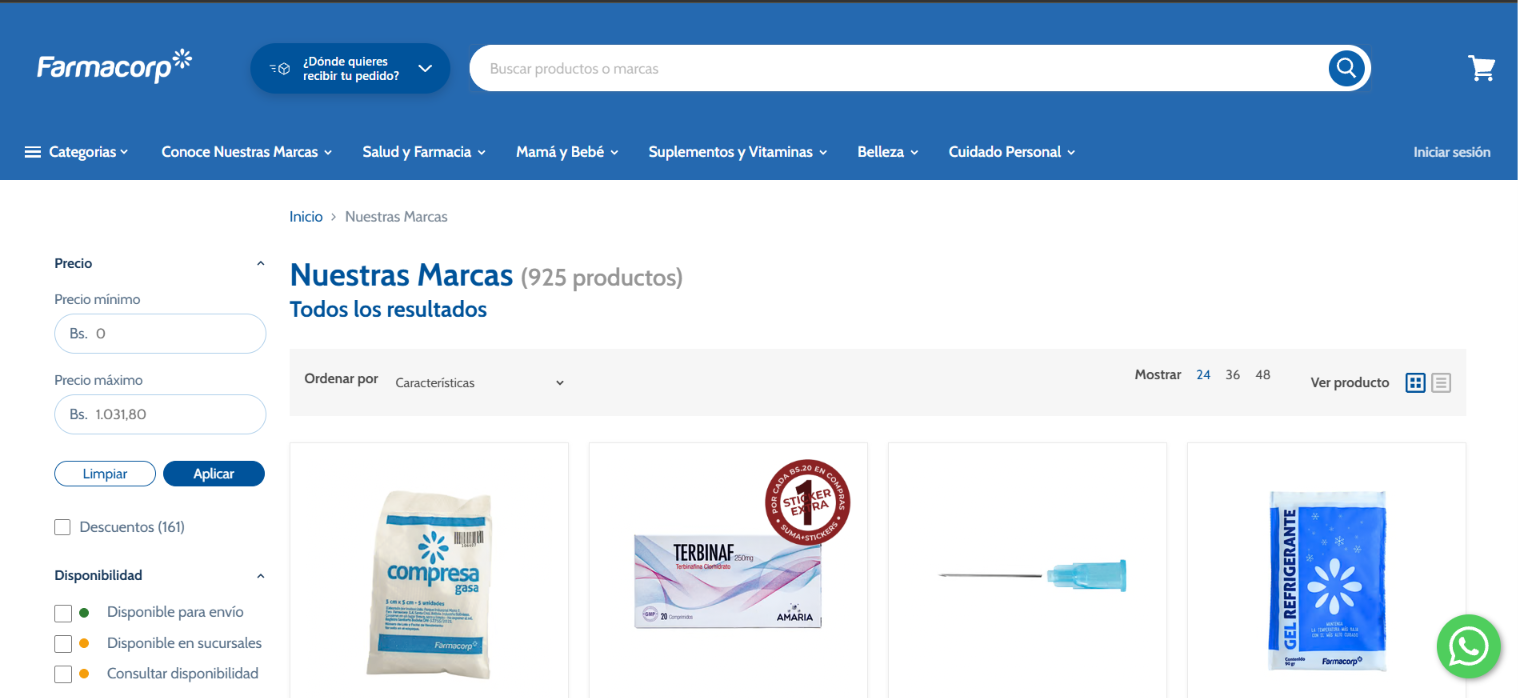
\includegraphics[width=\linewidth]{figuras/imgFarmacorpStore.png}
        \caption*{(a) Tienda digital Farmacorp (Shopify)}
    \end{minipage}\hfill
    \begin{minipage}{0.49\linewidth}
        \centering
        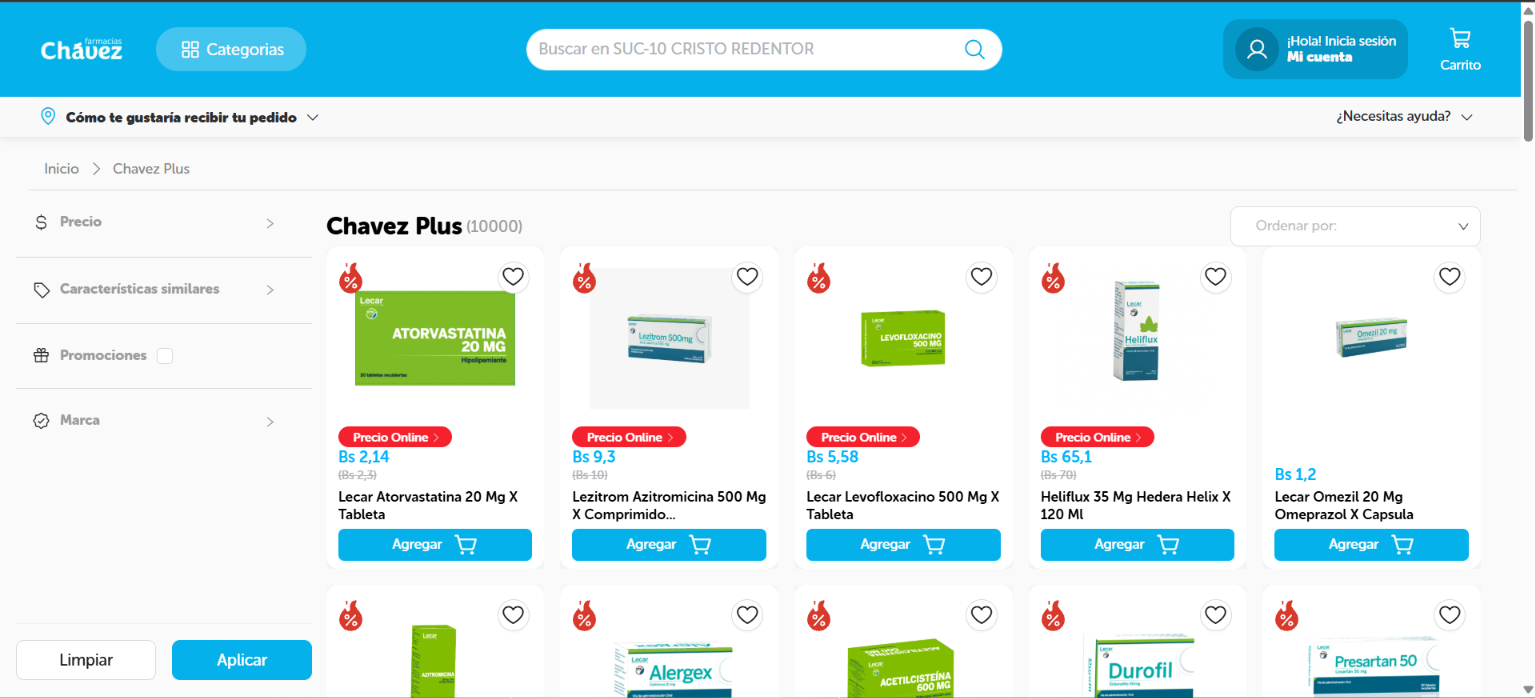
\includegraphics[width=\linewidth]{figuras/imgChavezStore.png}
        \caption*{(b) Tienda digital Farmacias Chávez (Next.js)}
    \end{minipage}
    \figurenote{Capturas de los portales comerciales de comercio electrónico de Farmacorp y Farmacias Chávez, evidenciando las estructuras de catálogo, banners promocionales y filtros facetados analizados por los scrapers.}
\end{figure}


% ----------------------------------------------------
% REFERENCIAS BIBLIOGRÁFICAS
% ----------------------------------------------------
\newpage
\phantomsection
\addcontentsline{toc}{section}{REFERENCIAS BIBLIOGRÁFICAS}
\bibliographystyle{apalike}
\bibliography{secciones/bibliografia}

\end{document}
